\documentclass[a4paper,12pt]{article}
\usepackage{blindtext}
\usepackage[utf8]{inputenc}
\usepackage{hyperref}
\usepackage{graphicx}
\usepackage{float}
\graphicspath{ {images/} }

\begin{document}

\begin{titlepage}

\newcommand{\HRule}{\rule{\linewidth}{0.5mm}} % Defines a new command for the horizontal lines, change thickness here

\center % Center everything on the page
 
%----------------------------------------------------------------------------------------
%-	HEADING SECTIONS
%----------------------------------------------------------------------------------------

\textsc{\LARGE University of Pretoria}\\[1.5cm]
\textsc{\Large COS 301 - Software Engineering}\\[0.5cm]
\textsc{\large Team Fox}\\[0.5cm]

%----------------------------------------------------------------------------------------
%-	TITLE SECTION
%----------------------------------------------------------------------------------------

\HRule \\[0.4cm]
{ \huge \bfseries Software Requirements Specification and Technology Neutral Process Design}\\[0.4cm] % Title of your document
\HRule \\[1.5cm]
 
%----------------------------------------------------------------------------------------
%-	AUTHOR SECTION
%----------------------------------------------------------------------------------------

\begin{minipage}{0.4\textwidth}
\begin{flushleft} \large
\emph{Author(s):}\\
Gian Paolo \textsc{Buffo}\\ % Your name
Jita \textsc{Hlengekile}\\
Jacques \textsc{van Wyk}\\
Jedd \textsc{Schneier}\\
Jason \textsc{Gordon}\\
Josef \textsc{Alberts}\\
Sandile \textsc{Khumalo}\\
Kudzai \textsc{Muranga}
\end{flushleft}
\end{minipage}
~
\begin{minipage}{0.4\textwidth}
\begin{flushright} \large
\emph{Student number(s):} \\
14446619\\ % Student number
14077893\\
12230091\\
13133064\\
14405025\\
14395283 \\
12031748\\
13278012
\end{flushright}
\end{minipage}\\[4cm]


%----------------------------------------------------------------------------------------
%-	DATE SECTION
%----------------------------------------------------------------------------------------

{\large \today}\\[3cm] % Date, change the \today to a set date if you want to be precise

 
%----------------------------------------------------------------------------------------

\vfill % Fill the rest of the page with whitespace

\end{titlepage}

\newpage

%=========================================READ ME========================================
%----------------------------------------------------------------------------------------
% I have randomly assigned questions to all of us to get the ball rolling. Obviously,
% anyone can contribute to anything if they feel they have something to add/change.
% The names will be above each section.
% - GP
%----------------------------------------------------------------------------------------

\tableofcontents

\newpage

%----------------------------------------------------------------------------------------
% Done by: Jason Gordon
%----------------------------------------------------------------------------------------
\section{Introduction}

This is the Software Requirements specification document for the system to keep record of research papers in the Computer Science Department of the University of Pretoria.
This document includes sections such as:
\begin{enumerate}
    \item Vision for the system
\begin{itemize}
    \item This includes the projected vision and outcomes of the system and what the Computer Science Department aims to achieve with this project. 
\end{itemize}

    \item Background to why the system is being developed

\begin{itemize}
    \item This includes a discussion of the problem which the Computer Science Department is faced with in regard to keeping track of their research papers and how this system will find a solution to the problem being faced. 
\end{itemize}

    \item Architecture Requirements
\setlength{\parindent}{2.5em}

\begin{itemize}
    \item This includes how the system will be accessed by the users of the system and through which platforms this will be done. Additionally the quality requirements of the system will be discussed as well as what external systems will be used to put this system together. Lastly it will include any constraints that the client has specified with regard to what must be used in the system. 
\end{itemize}

    \item Functional requirements and application design

\begin{itemize}
    \item This will include the functionality of the system that is required by the users of the system. 
\end{itemize}
    \item Open Issues
\begin{itemize}
    \item This section will discuss any requirements of the system that may be unclear or has not been specified. It will also include any inconsistencies that have been discovered in the requirements. 
\end{itemize}
\end{enumerate}

%----------------------------------------------------------------------------------------
% Done by: Gian Paolo Buffo
%----------------------------------------------------------------------------------------
\newpage
\section{Vision}

With the implementation of this system, the client is trying to create a central piece of software that can be used by all staff members of the Computer Science department of the University of Pretoria to maintain their academic publications.

However, the software will provide much greater functionality than merely listing all publications. One of the main features of the system will be the ability to add and edit publications, as well as specify a multitude of metadata items such as the title, (co)-authors, deadlines, progress towards completion, status (published, accepted, submitted etc.) and intended venue (conference, journal).

Additionally, the system will be used to provide users (who are authors of publications) with all manner of information regarding their Research Output Units and funding. This includes information such as expected units and funding, obtained units and funding, and shortfall of units.

The system will provide outputs in the form of an Excel spreadsheet which will illustrate the aforementioned author details both in a tabular fashion and graphically, most likely in the form of bar and/or line graphs. A sheet will be generated for each individual author, and a master sheet will be generated for the Research Leaders and Head of Department respectively.

A typical usage scenario of the system will be as follows:
\begin{itemize}

\item A user, who in this case is an author as well as the Head of Department (giving him/her administrator rights), logs in to the system.
\item The user then adds a new publication on his/her profile page, filling in the relevant metadata items. The user will by default be added as an author.
\item The user realises that he/she made an error while filling in the title, and edits the title appropriately.
\item The units corresponding to the publication's venue (which have been assigned by the system) are automatically added to the user, and all unit-related calculations are made
\item The user's profile page is updated with the new publication and all related information.
\item The user then chooses to generate the Excel document which contains not only information about his/her Research Output Units and funding in a tabular and graphical fashion, but also similar information for all other members of the department, who are users. This is because the user has Head of Department rights. 

\end{itemize}

%----------------------------------------------------------------------------------------
% Done by: Jacques van Wyk (edited by Gian Paolo Buffo)
%----------------------------------------------------------------------------------------
\section{Background}

Our group, Team Fox, had a meeting with the client, Ms Vreda Pieterse, on Wednesday, 17 February 2016. The client discussed that she requires the implementation of a system which will allow researchers to keep track of their publications, as well as view statistical information regarding their Research Output Units.

We have been given this topic for our mini project for the module COS 301. Furthermore, the mini project is to train us and help assist us in readying ourselves for the main project of this module.

This will give our group, Team Fox, the opportunity to gain experience on how to put together an SRS (Software Requirements Specification) that will help us and the client to better understand what is needed from the system and its functionality and how they would like to interact with the system. Consequently, if we better understand what our client wants the system to be, it will give us a better opportunity to implement a system that the client will be pleased with and which the client will want to use.
 	
In addition, the system will be used by the Computer Science department at the University of Pretoria. Hopefully the system will improve on the system(s) currently in use and will provide a basic structure of good quality which will enable it to be updated and improved in the future of its software development life cycle.
 	
Furthermore, the project might serve as an example to other students on how to implement such a system or it can be used as a basic structure and starting point for other institutes.

\newpage
\section{Architecture Requirements}

The software architecture requirements include the access and integration requirements, quality requirements and architectural constraints. We will return to the software architecture again toward the end of the paper.

%----------------------------------------------------------------------------------------
% Done by: Kudzai Muranga (edited by Gian Paolo Buffo)
%----------------------------------------------------------------------------------------
\subsection{Architectural Scope}
The system will allow the staff of the Computer Science department to keep a record of their research publications.
It will allow the staff to add and remove papers on the system as well as add and edit the metadata about each publication.
The system will allow users to view other user's profiles for when they need their details in order to add them as authors to their publications.

The system will send notifications to the users when their publications are reaching their deadlines. It will send these notifications via email.

The information that the system uses, such as the papers and their metadata and authors will be stored using a MongoDB database.

An Excel spreadsheet will be used for reporting purposes. It will list the staff members, their publications, the number of units allocated to each staff member, as well as budget information.

%----------------------------------------------------------------------------------------
% Done by: Hlengekile Jita (edited by Gian Paolo Buffo)
% TO BE EXTENDED ACCORDING TO NEW TEMPLATE
%----------------------------------------------------------------------------------------
\subsection{Access Channel Requirements}

When considering the access channels of a target system, there are two main possibilities to consider: the human users of the system and whether any other systems need to be able to access the system. For both of these possibilities one then needs to consider through which ways they will access the system, what functionality the system requires these access channels to have and how these access channels will provide said functionality. 

The system required by our client (which will from herewith be referred to as the system or the target system) is a system through which researchers can keep track of their publications. The users of the system, the researchers, need a channel through which they can use the system. The client does not require any other systems to be able to access our system or use the functionality of our system for a higher processing scheme, at this stage.

The client would like the creation of two platforms through which the users of the system can access the system, namely:
\begin{itemize}
	\item A Web Interface
	\item A Mobile Application (On the Android platform)
\end{itemize}

Both of these will have to access our system through the Internet - for the Android Application, this will require requesting permissions. The aforementioned platforms will need an interface through which to access our system, known as an Application Programming Interface (API). This interface will have to enable the passing of data from the system to the channel through which the user accesses the system. Considering the general functionality our system provides, and that communication would take place through the Internet, this API would have to be RESTful.

REST stands for Representational State Transfer, and it is a software architectural style that deals with resources and what resources are accessed through using the HTTP user-oriented network protocol. This RESTful API would enable the transfer of data between our system and the platforms our client has chosen for users to access the system through - in our case over a network, namely the Internet.

Before we consider this API further and what data it shall pass and how our access channels will use the API, let us revisit the functionality the access platforms will need to have to provide the users with the target system's maximum functionality.
\begin{itemize}
	\item User log in
	\item Search functionality
	\item Ability to open excel spreadsheets
	\item Viewing of plain text
	\item Viewing of lists, tables etc.
	\item Viewing of links
	\item Ability to view information
	\item Ability to add information
	\item Ability to change information
	\item Ability to remove information
\end{itemize}

For the viewing of text, lists, links and the like, this will have to do with the Graphical User Interface (GUI) that the access channel provides. In the case of the Web Interface this can be designed using HTML and its associated counterparts such as CSS, Bootstrap and more. In the case of the Android Application, a number of classes and functions will be used. For example in the case of a list, one would use a ListView item on their user interface and this can be created using the android.widget.ListView class, and operations on said list will be done using the classes' associated functions.

The Search functionality would also need to be provided by the Graphical User Interface, but actual searching of the database used in our system will be done by the system itself, so our API would need to be able to request the system to do the search, when a user provides the required information for the search by interacting with the GUI.

For the ability to open Excel spreadsheets, in the Web Interface, this would imply the ability to download a file; while on an Android Application, this would imply the same thing as well as the improved ability to open the user devices' spreadsheet viewer.

As for the user log in functionality, users would provide user details through the GUI and the API would then need to pass user details for verification to the system and be able to receive a response about whether or not log in was successful or not. Another option that would be safer is the use of API authentication, this is a token based authentication in which the user would log in and if successful the system will respond with a unique token that can be used in future requests.

As we already know the information that will be displayed on these platforms GUIs will be provided through the RESTful API from our system. For this information, the API would need to get information from the system and be able to send changes including the addition and removal of information back to the system. Basically all the interaction between the system and these platforms will be done by the API with the following HTTP methods:
\begin{itemize}
	\item GET – For reading information from the system
	\item PUT – For adding information to the system
	\item DELETE – For removing information from the system
	\item POST – For making changes/edits to information on the system
	\item OPTIONS – For getting operations that can be performed by the system
\end{itemize}

While these platforms vary, they will both access the system through this API and use the Internet to communicate with the system. However the ways they call the API, process and deal with the responses will vary slightly on the two platforms. The API would provide a standard way for accessing the system despite what channel may be in use. These access channels thus simply need to provide users with the functionality that the target system requires on a GUI and use the API for providing users with the results and information from the system.
\\\\
\textbf{References}
\begin{itemize}
\item \url{http://www.andrewhavens.com/posts/20/beginners-guide-to-creating-a-rest-api/}
\item \url{http://www.tutorialspoint.com/restful/restful_introduction.htm}
\end{itemize}

%----------------------------------------------------------------------------------------
% Done by: Josef Alberts (edited by Gian Paolo Buffo)
% TO BE EXTENDED ACCORDING TO NEW TEMPLATE
%----------------------------------------------------------------------------------------
\subsection{Quality Requirements}

\subsubsection{Performance}
The system must work as efficiently as possible and not lag in delivering information to the user. Since this system will not be sending large amounts of data, it should not be difficult for the system to transfer the data speedily. In this implementation, we expect the network speed to dictate performance – not the system itself. Regardless, the system must be able to handle the full amount of users (approx. 100) concurrently without experiencing significant delays or errors. The success of this requirement can be measured in the time taken for a task to be completed under normal, and heavy-load scenarios

\subsubsection{Reliability}
It is imperative that the system not experience unnecessary downtime (period of in-operation of the system), thus preventing users from checking on or altering information on the system. An optimal uptime (period of normal operation of the system) within a month would be 99\% and upwards. Additionally there should not be frequent errors within normal operating parameters of the system. This means that simple logins (sessions), alterations or additions to the database should not cause errors which affect the system as a whole. Additionally, minor human errors, such as omission of information, should not be allowed to propagate through the system. But the system should rather allow the user to fix the error immediately – which will also contribute towards the accuracy of information in the database.

\subsubsection{Scalability}
The system will initially be implemented to manage papers pertaining to one faculty, but it might be necessary in the future to expand it to manage more faculties. The maximum amount for one implementation to manage should not exceed 11, and as such it should be scalable to that amount of faculties and the users associated with them. We make the assumption that the total users per faculty does not exceed 100 and, thus, the total on the system will never exceed 1100.

\subsubsection{Usability} 
Users must be able to login, edit information and logout without hassle. The interface should not be cluttered and should not contain redundant information. As management of information on the system is critical, accessing said information should be as simple as possible.

\subsubsection{Auditability}
In order to track changes and/or errors on the system, all actions by users must be logged as they occur. This includes, but is not limited to, log-in attempts, editing of information (whether successful or not) and log-outs. All errors should also be logged in order to simplify error-tracking. The logging system must not interfere with the users' actions and must not significantly affect performance. Logs must be timestamped and must contain information on which user executed an action – or where an error occurred.

\subsubsection{Security}
The system will be protected by a login system which will require a user to enter an ID and a password. The ID and password will then be compared to users in the system's database and, if an appropriate user is found AND the passwords (entered and stored) match, may the user proceed to access the system. This system must not, under any circumstances, allow unauthorised users to enter the system. If a user enters incorrect information, the system must notify the user and request that they correct the input before allowing them to continue to the rest of the system.

%----------------------------------------------------------------------------------------
% Done by: Jedd Schneier (edited by Gian Paolo Buffo)
% TO BE EXTENDED ACCORDING TO NEW TEMPLATE
%----------------------------------------------------------------------------------------
\newpage
\subsection{Integration Requirements}

As the system will be accessed remotely through the Internet, it needs to integrate with web services. The GUI will be integrated online with HTML, JavaScript, CSS and any frameworks or libraries the developer decides to use as long as the system itself remains compatible on all browsers and does not use browser-exclusive functionality. The system must be integrated with the server, and thus make use of appropriate server-side technology such s AJAX and PHP. In summary, the system needs to be accessed anywhere on any browser through any device regardless of screen resolution, computer Operating System or hardware specification. Additionally, the system must work with these technologies in a robust and consistent manner. 

For mobile development, the system is required to integrate with the Android mobile Operating System. It must work correctly on all previous versions, and thus have no dependency on current feature sets. It must also be scalable to future Android releases and switching from account access through Android to web access and vice versa must be seamless and secure. On that note, the system must integrate well with security measures.

Externally, the system must be integrated with a database system such as LDAP, mongoDB or an appropriate alternative the developer decides on, provided that the system integrates with the database securely and it remains scalable. The system is also required to send emails to users, and thus it must have email integration either through external email servers or technologies, or an internally created one. Any libraries or packages needed to realise the functional requirements must be integrated with the other technologies being used. It was decided that the system does not need to integrate with Google Calender and thus it will not be using the Google API.

The system will generate reports in the form of spreadsheets and this must be integrated with the appropriate technology such as Microsoft Excel or LibreOffice Calc. The system will also regularly generate statistics and graphs so it is imperative the system integrates with statistical modelling technologies. As the system will be primarily an Internet-based application, the HTTP protocol suite will be primarily used for website data passing from client to server. The sending of emails should adhere to the SMTP suite and message passing through the system can be achieved through TCP. 

All integration needs to be seamless and not interfere with system performance. Security is also a major concern, and thus technologies integrated must not threaten the system's security as a whole or other technologies. The system must remain portable to any Android device and to any browser. As the system may grow and shrink as users are added and deleted, the system must be scalable. The data stored in the system will also increase and thus storage integration must be scalable as well. The system must remain reliable with each integrated technology added, and any errors must be able to be traced to the technology causing it.

%----------------------------------------------------------------------------------------
% Done by: Jason Gordon
% TO BE EXTENDED ACCORDING TO NEW TEMPLATE
%----------------------------------------------------------------------------------------
\subsection{Architecture Constraints}

There are not too many architectural constraints to this system. However some constraints do exist, such as:
\begin{itemize}
\item The only technological constraint we have been given is the fact that we cannot link the system to any external resources besides for sending an email reminder, to the user, about the due date for their paper.
	\begin{itemize}
	\item The only constraint with regard to this would be that we would not be able to ease the way in which the user could keep track of their due dates by \textit{e.g. Adding the date directly to their google calendar}. Thus the user would manually need to add the date to their calendar or create a reminder for themselves (if they want to). Another problem could be that the email reminder that is sent by the system could be cluttered between all the other emails that have been received, by the user, and thus the user may forget about the reminder that was sent by the system. 
	\end{itemize}
\item The role of the user in the system \textit{(i.e. Author, Research Leader, Administrator, Head of Department)} determines their permissions on the system.
	\begin{itemize}
	\item Author - May only edit metadata about a paper they are working on or have already published.
	\item Research Leader - May see all papers in his or her research group.
	\item Administrator/Head of Department - Should be able to view everything in the system (including all papers published, in progress or discontinued) as well as the number of units each user has earned. They may also add or remove users.
	\end{itemize}
\item The system must only cater for the Computer Science Department of the University of Pretoria. Users may not be anyone else outside the department. 
\item When viewing profiles of other users, one may not see the papers of the other users - despite the progress of these papers - or the number of units they have earned in total. 
\item However when viewing ones own profile, one may view their papers - regardless of progress - and also may view the number of units they have earned in total. 
\item Developing the system for the web can be very different from developing it for Android. This does, however, depend on the language(s) used to develop the Android application. If it is coded using web based languages it would be easier to port it to android. However if it is developed using Java the web-based system would not be very portable to Android. 
\item Additionally if this system ever needed to be ported to other mobile OS's such as iOS or Windows Mobile it would be difficult due to the difference in development language for each OS.
\item Lastly no papers, once added, may be deleted. Thus the database could become very large and make system backup and restore more difficult. Also there is no automatic backup of the data in the system, thus it would need to be done manually. 
\end{itemize}

We will return to the software architecture requirements again later on in the paper. 

\newpage
\section{Functional requirements and application design}
This section discusses the application functionality required by users (and other stakeholders).

%----------------------------------------------------------------------------------------
% Done by: Sandile Khumalo (edited by Gian Paolo Buffo)
%----------------------------------------------------------------------------------------
\subsection{Use case prioritization}
Critical
\begin{itemize}
\item Adding a conference paper
\item Adding an author to a conference paper
\item User being able to see all papers they have added or co-authored
\item Adding a researcher to a research group
\item Editing publication metadata 
\item Research leader being able to view all papers and their progress
\item The state of the paper (submitted, waiting, rejected, published)
\item Functionality to back up information 
\item Add and remove authors any time of the paper
\item Show history of papers
\item Staff members being able to access the portal

\end{itemize}
Important
\begin{itemize}
\item Head Of Department being able to view all papers
\item The sequence of authors(primary,second etc.)
\item Log all activity 
\item Keep track of units, showing charts to see if authors meet the target
\item Count units only when paper has been published
\item U.P. is the default occupational address of all papers
\item Show the intend venue of papers and the type of the paper
\item Send a reminder of when the paper is due
\item Units allocated to each venue appear by default once they has been stored
\item Search for an author
\item Head of department being able to view all units for all staff members
\item An Administrator having complete access to the portal even on behalf of other users
\item Head of Department having complete access to the portal even on behalf of other users
\end{itemize}
Nice to have
\begin{itemize}
 \item Profile of the researcher
 \item Scalability to provide functionality for multiple departments
 \item A user who is not an author adding a paper for someone else
\end{itemize}

%----------------------------------------------------------------------------------------
% Done by: Kudzai Muranga (edited by Gian Paolo Buffo)
%----------------------------------------------------------------------------------------
\newpage
\subsection{Use case/Services contracts}
Adding a conference paper:
\begin{itemize}
    \item Preconditions
    \begin{itemize}
        \item User must be a staff member
        \item User must be logged in
        \item A paper must have at least one author
         \item Primary author must be specified
        \item User must enter the metadata about the paper
    \end{itemize}
    \item Postconditions
    \begin{itemize}
        \item Conference paper successfully added
    \end{itemize}
    \item Exceptions
    \begin{itemize}
        \item User can create a paper but does not have to be an author
    \end{itemize}
    
    \begin{figure}[H]
    \centering
    \caption{Adding a conference paper}
    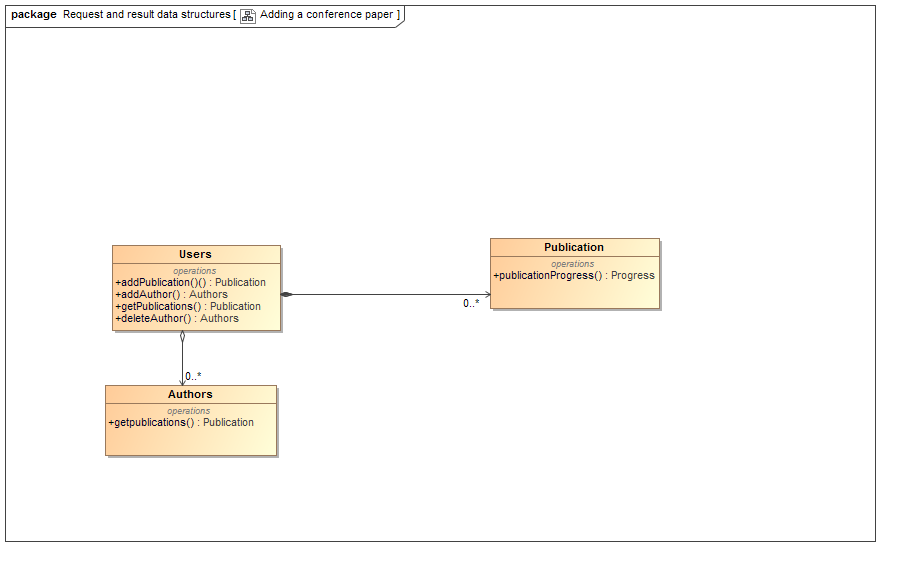
\includegraphics[width=1\textwidth]{use-case/adding-a-conference-paper.png}
    \end{figure}
\end{itemize}
\newpage
Adding an author to a conference paper:
\begin{itemize}
    \item Preconditions
    \begin{itemize}
        \item User must be a staff member
        \item User must be logged in
        \item User can specify the number of co-authors
    \end{itemize}
    \item Postconditions
    \begin{itemize}
        \item Author would be added to a paper
    \end{itemize}
    \item Exceptions
    \begin{itemize}
        \item Author does not have to be a user
    \end{itemize}
    
    \begin{figure}[H]
    \centering
    \caption{Adding an author to a conference paper}
    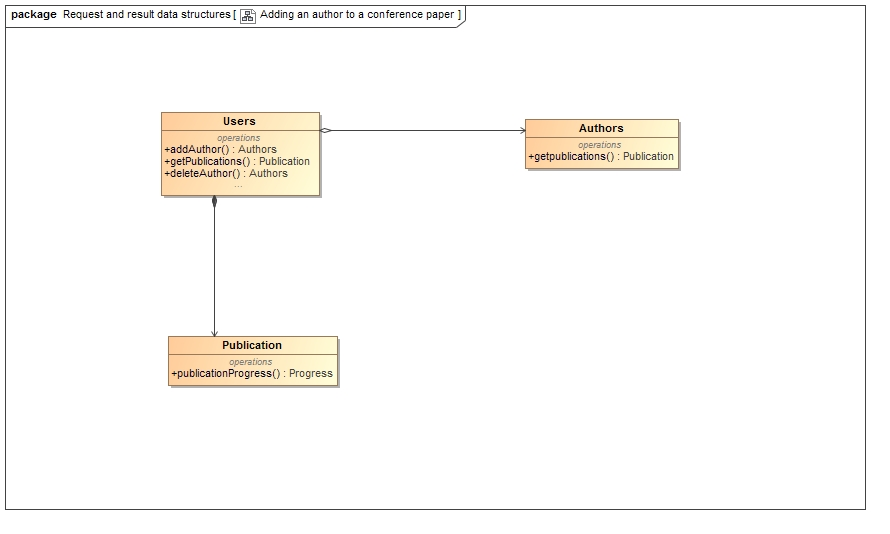
\includegraphics[width=1\textwidth]{use-case/adding-an-author-to-a-conference-paper.png}
    \end{figure}
\end{itemize}
User being able to see all papers they have added or co-authored:
\begin{itemize}
    \item Preconditions
    \begin{itemize}
        \item User must be logged in
        \item User must be an author or co-author to at least one paper
    \end{itemize}
    \item Postconditions
    \begin{itemize}
        \item User will be able to view their papers
    \end{itemize}
    
    \begin{figure}[H]
    \centering
    \caption{Users being able to view all authored/co-authored papers}
    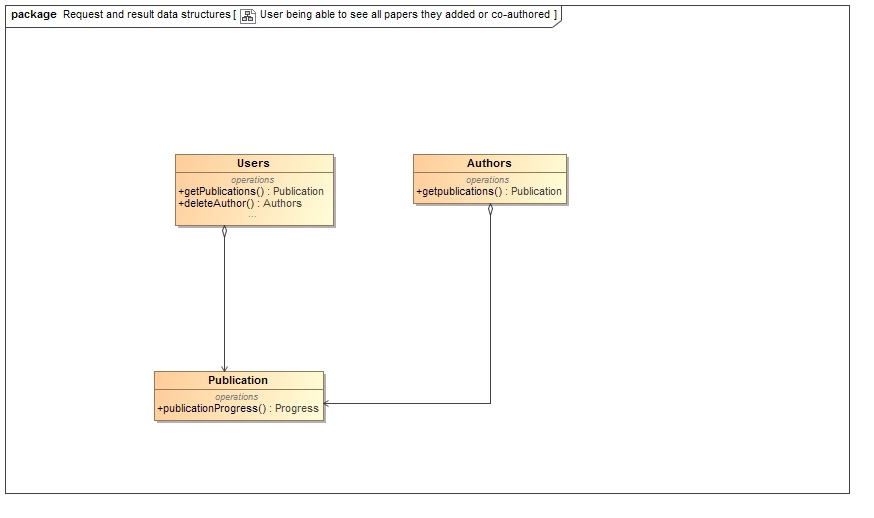
\includegraphics[width=1\textwidth]{use-case/user-viewing-papers.png}
    \end{figure}
\end{itemize}
Adding a researcher to a research group:
\begin{itemize}
    \item Preconditions
    \begin{itemize}
        \item User adding the researcher must be a researcher leader, Head of Department or an administrator
    \end{itemize}
    \item Postconditions
    \begin{itemize}
        \item Researcher added to research group
    \end{itemize}
    
    \begin{figure}[H]
    \centering
    \caption{Adding a researcher to a research group}
    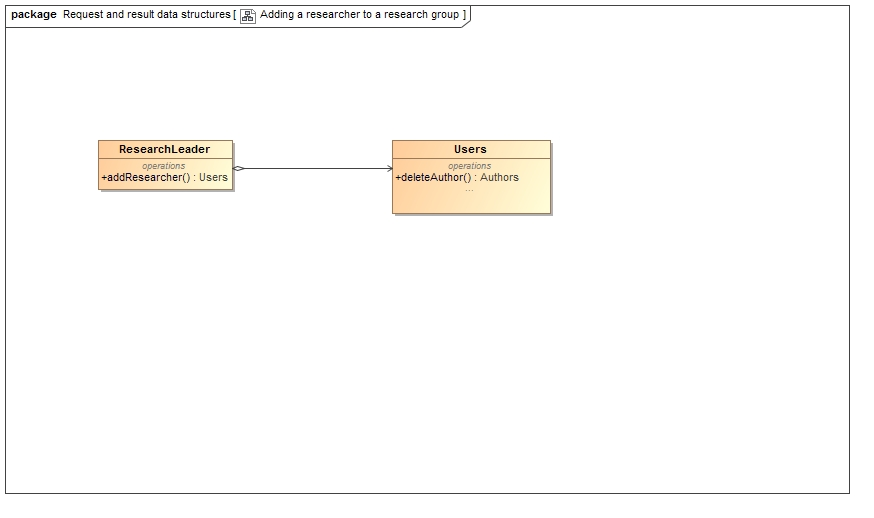
\includegraphics[width=1\textwidth]{use-case/adding-a-researcher-to-a-research-group.png}
    \end{figure}
\end{itemize}
The state of the paper (submitted, waiting, rejected, published):
\begin{itemize}
    \item Preconditions
    \begin{itemize}
        \item The paper must have already been added to the system
    \end{itemize}
    \item Postconditions
    \begin{itemize}
        \item The user can view the status of the paper
    \end{itemize}
    
    \begin{figure}[H]
    \centering
    \caption{Viewing the current paper state}
    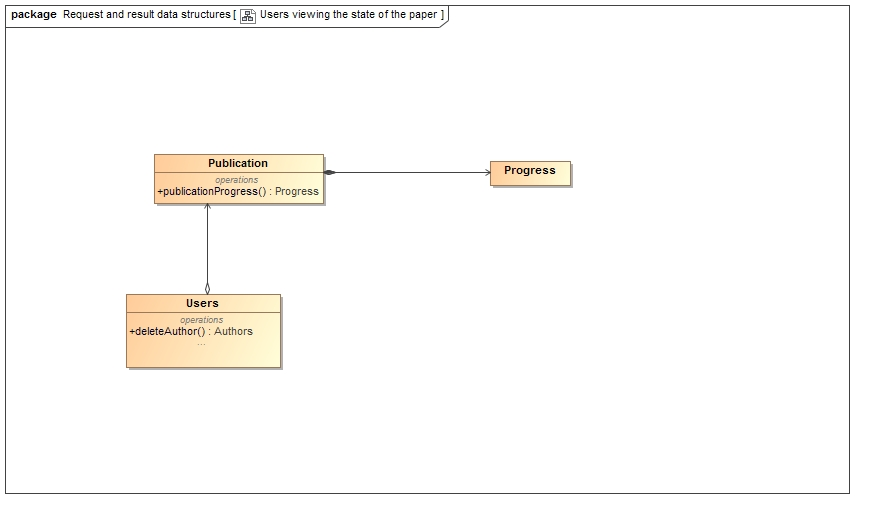
\includegraphics[width=1\textwidth]{use-case/user-viewing-paper-state.png}
    \end{figure}
\end{itemize}
Editing metadata:
\begin{itemize}
    \item Preconditions
    \begin{itemize}
        \item The user must be the author or co-author of the paper
        \item The paper must already be added in the system
    \end{itemize}
    \item Postconditions
    \begin{itemize}
        \item The user is successful in editing the meta data of the paper
    \end{itemize}
    \item Exceptions
    \begin{itemize}
        \item An administrator can edit the meta data of any paper in the system
        \item The head of department can edit the meta data of any paper in the system
        \item A research leader can edit the meta data of any paper in their research group
    \end{itemize}
    
    \begin{figure}[H]
    \centering
    \caption{Editing metadata}
    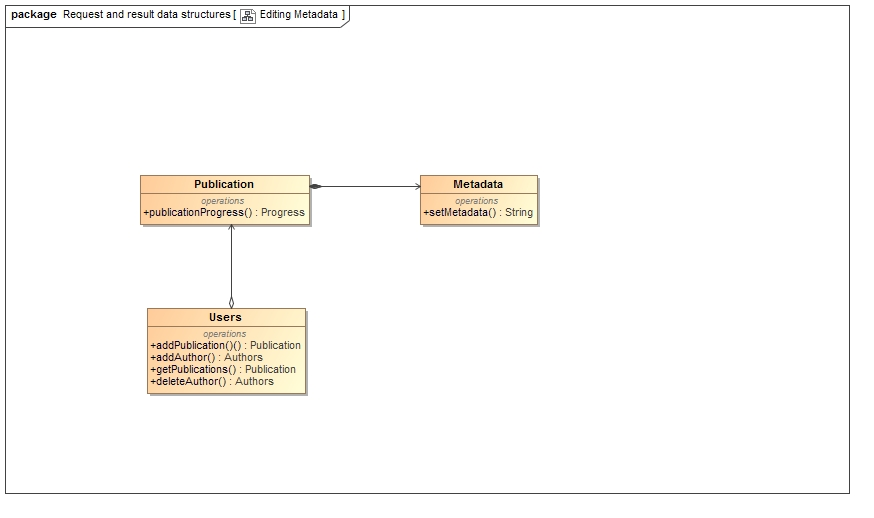
\includegraphics[width=1\textwidth]{use-case/editing-metadata.png}
    \end{figure}
\end{itemize}
Research leader being able to view all papers and their progress:
\begin{itemize}
    \item Preconditions
    \begin{itemize}
        \item The user must be the research leader of the research group
    \end{itemize}
    \item Postconditions
    \begin{itemize}
        \item The user will be able to view any paper in the research group
    \end{itemize}
    \item Exceptions
    \begin{itemize}
        \item The head of department and administrator can also view the papers in the research group
    \end{itemize}
    
    \begin{figure}[H]
    \centering
    \caption{Research leader being able to view relevant paper progress}
    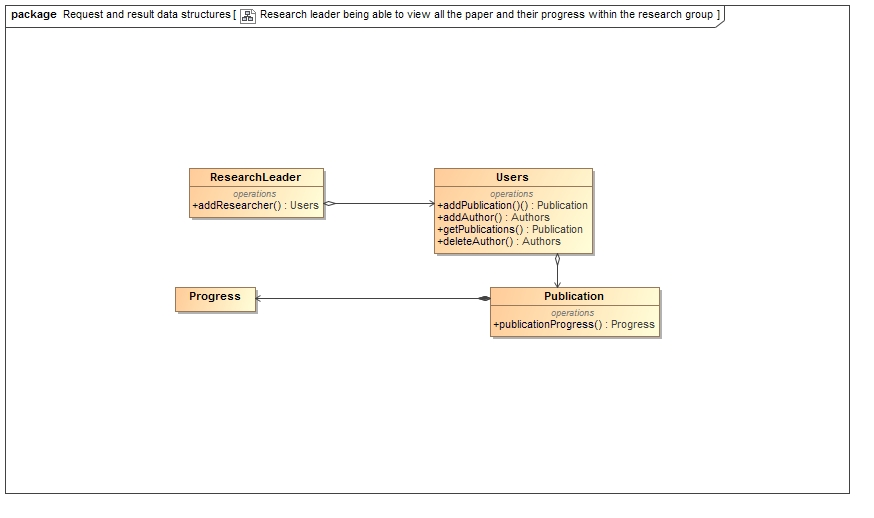
\includegraphics[width=1\textwidth]{use-case/research-leader-viewing.png}
    \end{figure}
\end{itemize}
Add and remove authors at any point in the life cycle of the paper:
\begin{itemize}
    \item Preconditions
    \begin{itemize}
        \item The user must be the primary author of the paper
    \end{itemize}
    \item Postconditions
    \begin{itemize}
        \item The user would be successful in adding or removing authors to or from the paper
    \end{itemize}
    
    \begin{figure}[H]
    \centering
    \caption{Adding and removing authors at any point in the life cycle of a paper}
    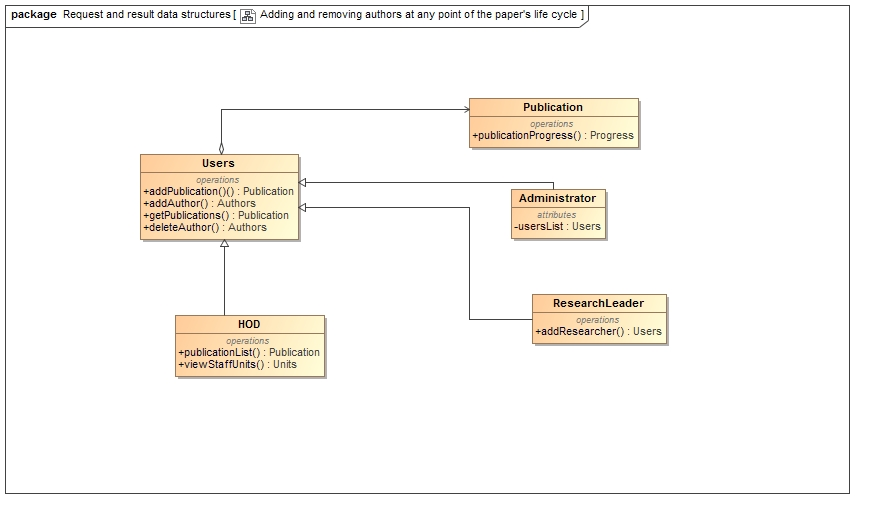
\includegraphics[width=1\textwidth]{use-case/adding-and-removing-authors.png}
    \end{figure}
\end{itemize}
Show history of papers:
\begin{itemize}
    \item Preconditions
    \begin{itemize}
        \item The user can only view the history of their own papers
    \end{itemize}
    \item Postconditions
    \begin{itemize}
        \item The user will successfully view their papers' history
    \end{itemize}
    \item Exceptions
    \begin{itemize}
        \item The head of department can view the history of any paper
        \item The administrator can view the history of any paper
        \item The research leader can view the history of any paper in their research group
    \end{itemize}
\end{itemize}
Staff members being able to access the portal:
\begin{itemize}
    \item Preconditions
    \begin{itemize}
        \item Staff members must have profiles on the system
    \end{itemize}
    \item Postconditions
    \begin{itemize}
        \item Staff members successfully access the portal
    \end{itemize}
    \item Exceptions
\end{itemize}
Head Of Department being able to view all papers:
\begin{itemize}
    \item Preconditions
    \begin{itemize}
        \item The user type must be the head of department
        \item There can only be one head of department
    \end{itemize}
    \item Postconditions
    \begin{itemize}
        \item The head of department can successfully view all papers
    \end{itemize}
    
    \begin{figure}[H]
    \centering
    \caption{H.O.D. being able to view all papers}
    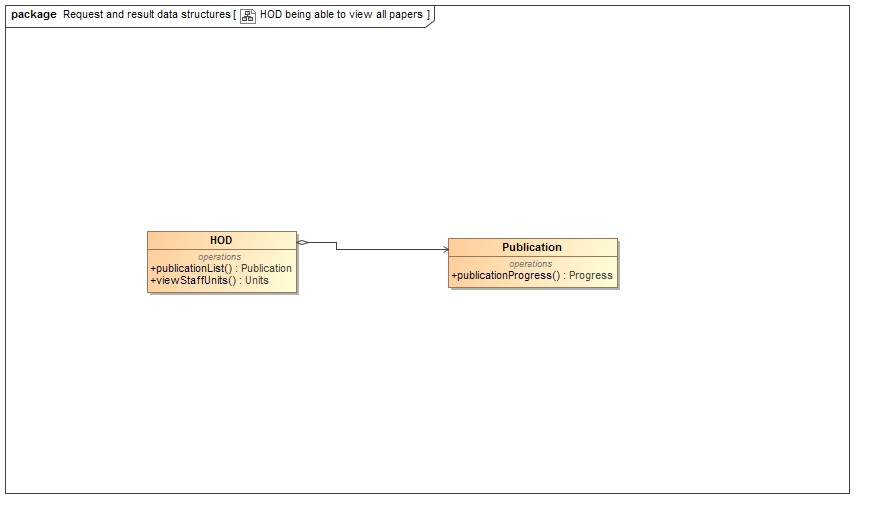
\includegraphics[width=1\textwidth]{use-case/hod-viewing-papers.png}
    \end{figure}
\end{itemize}
The sequence of authors(primary,second etc.):
\begin{itemize}
    \item Preconditions
    \begin{itemize}
        \item The sequence of authors must be specified by the user that created the paper
    \end{itemize}
    \item Postconditions
    \begin{itemize}
        \item The sequence of authors is specified
    \end{itemize}
\end{itemize}
Count units only when paper has been published:
\begin{itemize}
    \item Preconditions
    \begin{itemize}
        \item Units must be assigned to the paper
        \item Paper must already be published
    \end{itemize}
    \item Postconditions
    \begin{itemize}
        \item Units for the paper are counted
    \end{itemize}
\end{itemize}
U.P. is the default occupational address of all papers:
\begin{itemize}
    \item Preconditions
    \begin{itemize}
        \item A user profile must be in the process of being created
    \end{itemize}
    \item Postconditions
    \begin{itemize}
        \item The default institution for every profile will be U.p.
    \end{itemize}
\end{itemize}
Show the intended venue of paper and the type of the paper:
\begin{itemize}
    \item Preconditions
    \begin{itemize}
        \item Must be done by a user who is about to create a paper or edited by an author or co-author
    \end{itemize}
    \item Postconditions
    \begin{itemize}
        \item Intended venue and type of paper is shown
    \end{itemize}

\end{itemize}
Send a reminder of when the paper is due:
\begin{itemize}
    \item Preconditions
    \begin{itemize}
        \item User to be sent reminder must be an author or co-author of the paper
    \end{itemize}
    \item Postconditions
    \begin{itemize}
        \item Reminder is sent to the user about when the paper is due
    \end{itemize}
\end{itemize}
Venue units appear by default once they has been stored:
\begin{itemize}
    \item Preconditions
    \begin{itemize}
        \item User must specify the units allocated to the paper
    \end{itemize}
    \item Postconditions
    \begin{itemize}
        \item Units for the paper appear by default
    \end{itemize}
\end{itemize}
Search for an author:
\begin{itemize}
    \item Preconditions
    \begin{itemize}
        \item The author must be already added into the system
        \item The user searching for the author must be logged in
    \end{itemize}
    \item Postconditions
    \begin{itemize}
        \item The author is found if they exist
    \end{itemize}
\end{itemize}
Head of department being able to view all units per staff:
\begin{itemize}
    \item Preconditions
    \begin{itemize}
        \item User must be head of department
    \end{itemize}
    \item Postconditions
    \begin{itemize}
        \item head of department able to view the units allocated to each staff
    \end{itemize}
    
    \begin{figure}[H]
    \centering
    \caption{H.O.D. being able to view units per staff member}
    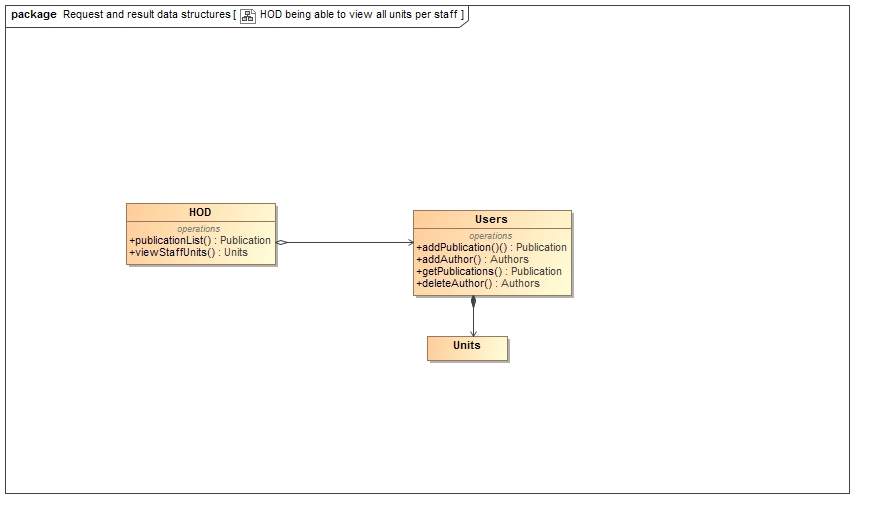
\includegraphics[width=1\textwidth]{use-case/hod-viewing-units.png}
    \end{figure}
\end{itemize}
An Administrator having complete access to the portal even on behalf of other users:
\begin{itemize}
    \item Preconditions
    \begin{itemize}
        \item The user must be an administrator
        \item The user the administrator is accessing must exist
    \end{itemize}
    \item Postconditions
    \begin{itemize}
        \item The administrator successfully have complete access to the portal
    \end{itemize}
    
    \begin{figure}[H]
    \centering
    \caption{An administrator having access to user profiles}
    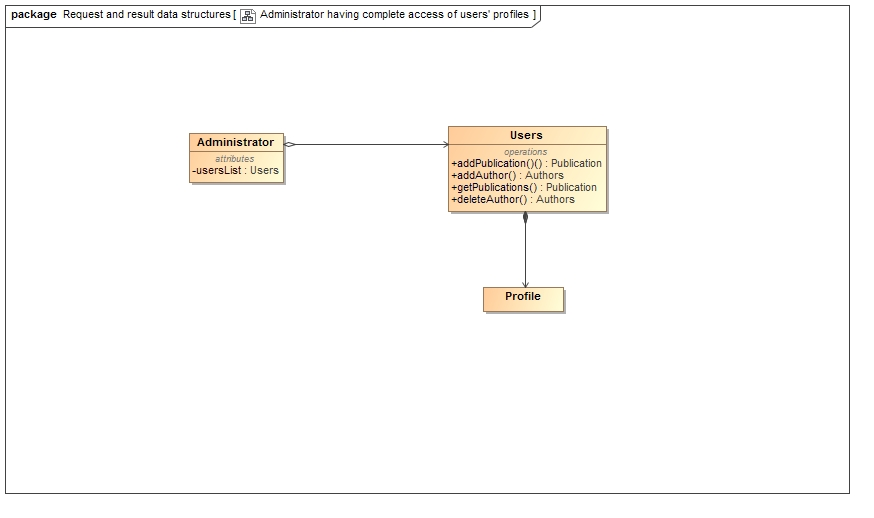
\includegraphics[width=1\textwidth]{use-case/administrator-access.png}
    \end{figure}
\end{itemize}
Profile of the researcher:
\begin{itemize}
    \item Preconditions
    \begin{itemize}
        \item The researcher must be logged in
        \item The researcher must already have a profile on the system
    \end{itemize}
    \item Postconditions
    \begin{itemize}
        \item The researcher can successfully view their profile
    \end{itemize}
\end{itemize}
A user who is not an author adding a paper for someone else:
\begin{itemize}
    \item Preconditions
    \begin{itemize}
        \item The user must be a staff member
    \end{itemize}
    \item Postconditions
    \begin{itemize}
        \item The user successfully creates a paper that another user is an author of
    \end{itemize}
\end{itemize}

%----------------------------------------------------------------------------------------
% Done by: Gian Paolo Buffo and Hlengekile Jita
%----------------------------------------------------------------------------------------
\newpage
\subsection{Required functionality}

This section describes the functionality required of the system, and illustrates these requirements by means of use case diagrams.

\begin{figure}[H]
    \centering
    \caption{Add a Paper}
    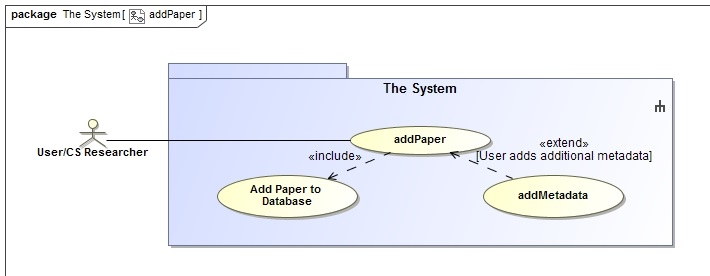
\includegraphics[width=1\textwidth]{req-func/uc__The_System__addPaper.jpg}
\end{figure}

\begin{figure}[H]
    \centering
    \caption{Add Metadata}
    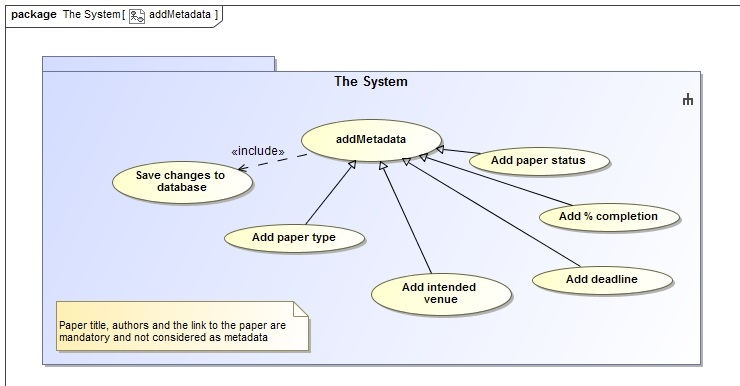
\includegraphics[width=1\textwidth]{req-func/uc__The_System__addMetadata.jpg}
\end{figure}

\begin{figure}[H]
    \centering
    \caption{Edit Paper Data}
    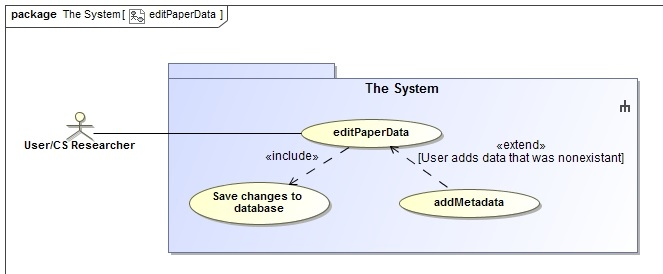
\includegraphics[width=1\textwidth]{req-func/uc__The_System__editPaperData.jpg}
\end{figure}

\begin{figure}[H]
    \centering
    \caption{View Authored Papers}
    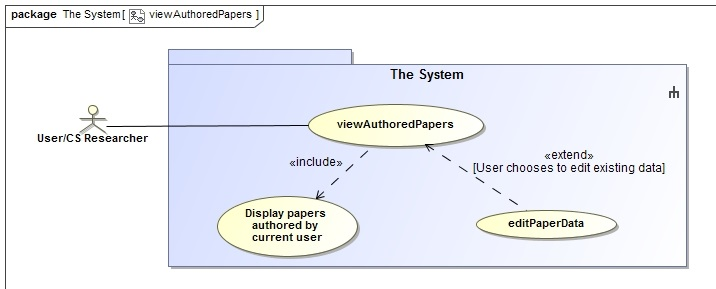
\includegraphics[width=1\textwidth]{req-func/uc__The_System__viewAuthoredPapers.jpg}
\end{figure}

\begin{figure}[H]
    \centering
    \caption{View Research Group Papers}
    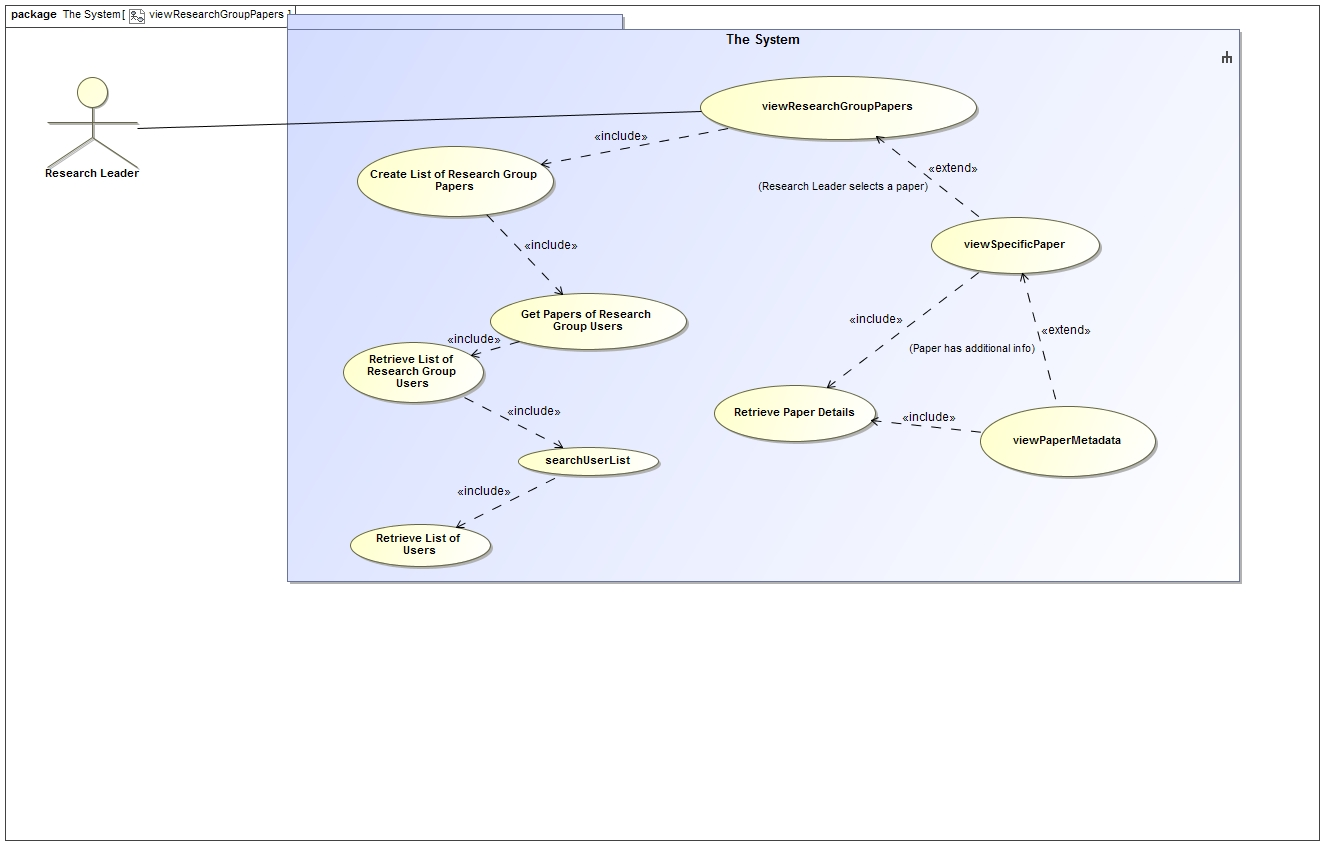
\includegraphics[width=1\textwidth]{req-func/uc__The_System__viewResearchGroupPapers.jpg}
\end{figure}

\begin{figure}[H]
    \centering
    \caption{View All Papers}
    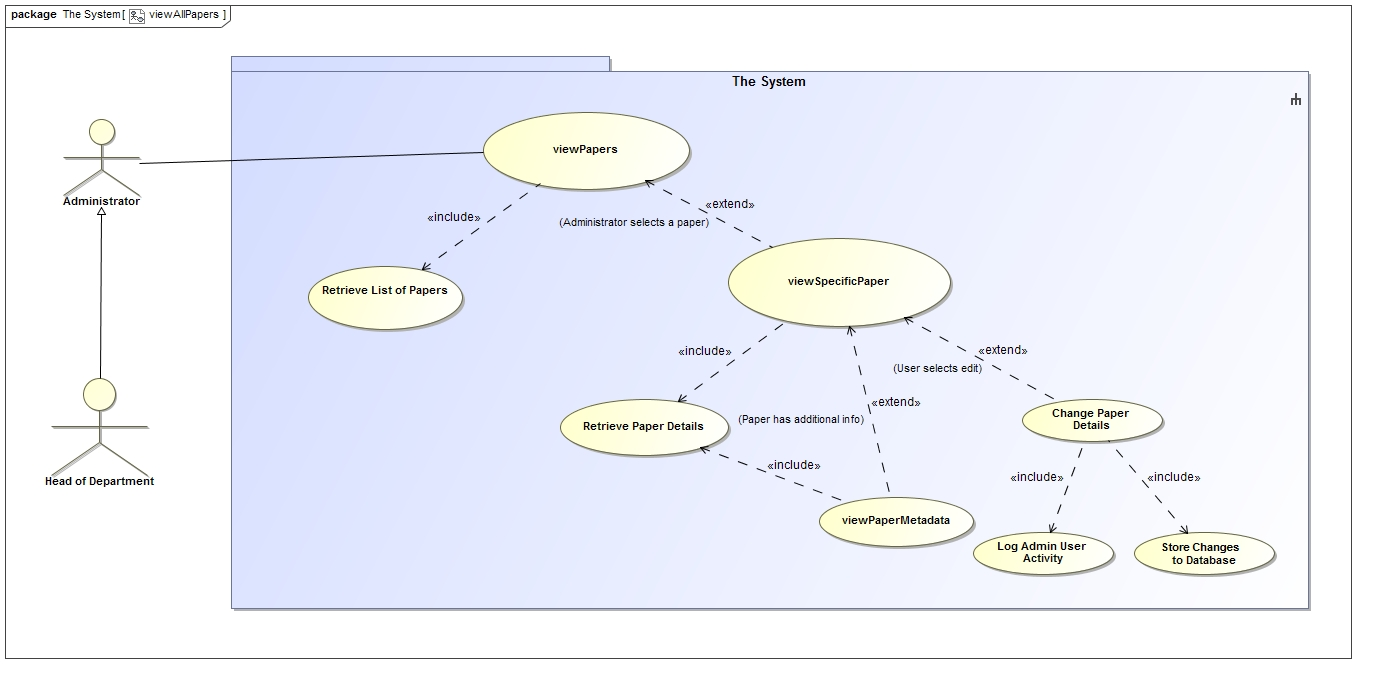
\includegraphics[width=1\textwidth]{req-func/uc__The_System__viewAllPapers.jpg}
\end{figure}

\begin{figure}[H]
    \centering
    \caption{Add User}
    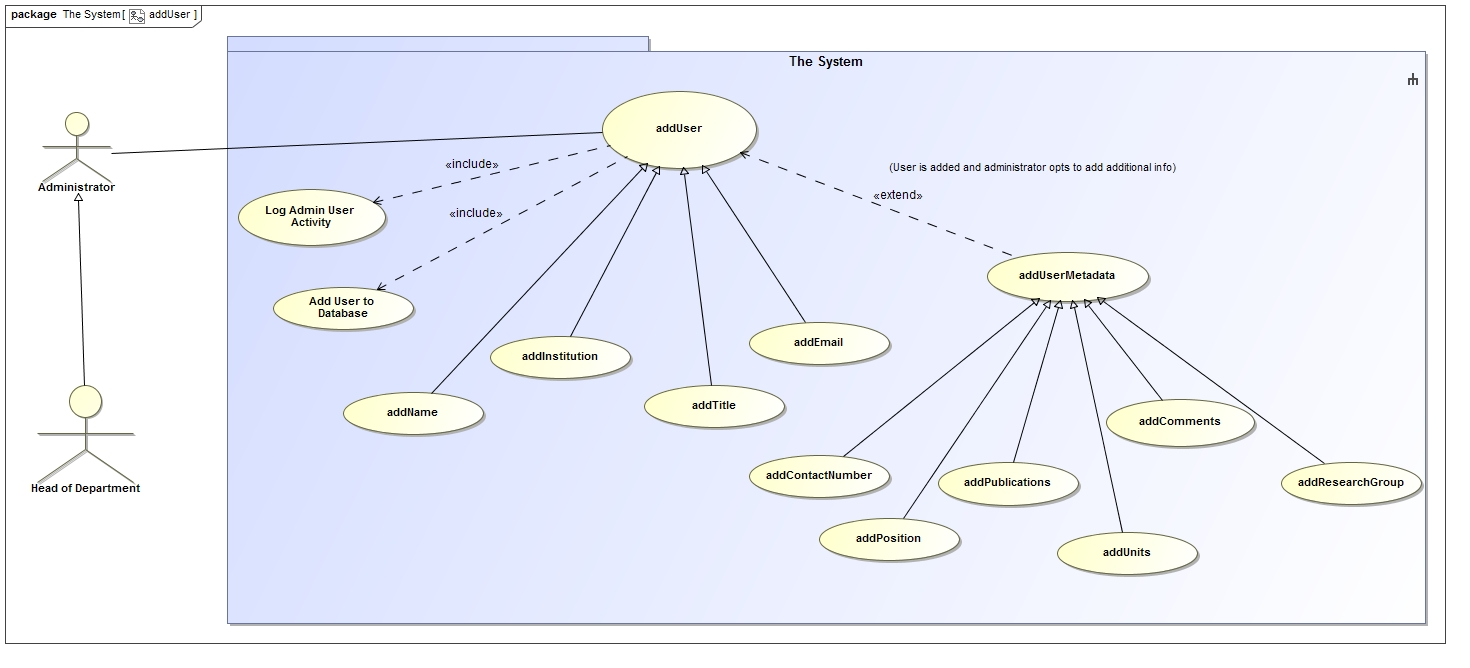
\includegraphics[width=1\textwidth]{req-func/uc__The_System__addUser.jpg}
\end{figure}

\begin{figure}[H]
    \centering
    \caption{Remove User}
    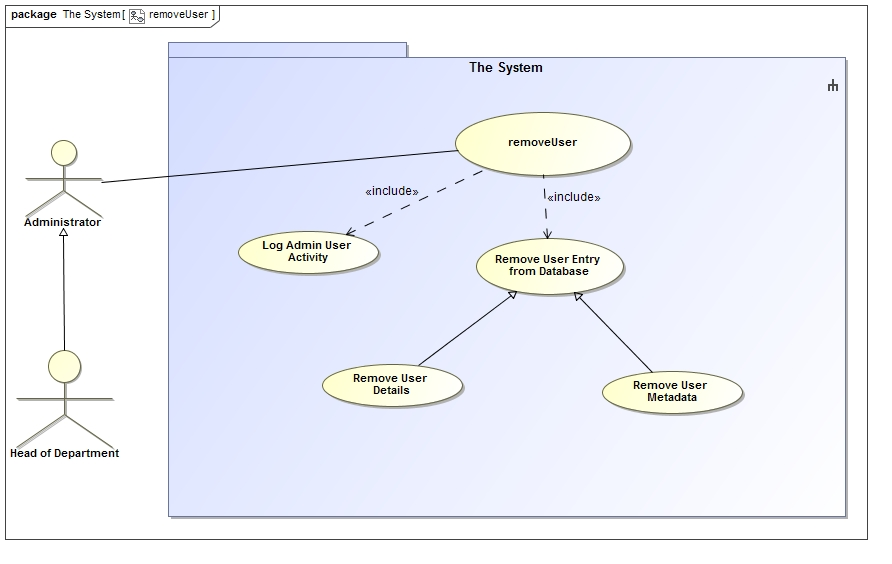
\includegraphics[width=1\textwidth]{req-func/uc__The_System__removeUser.jpg}
\end{figure}

\begin{figure}[H]
    \centering
    \caption{Add Research Group User}
    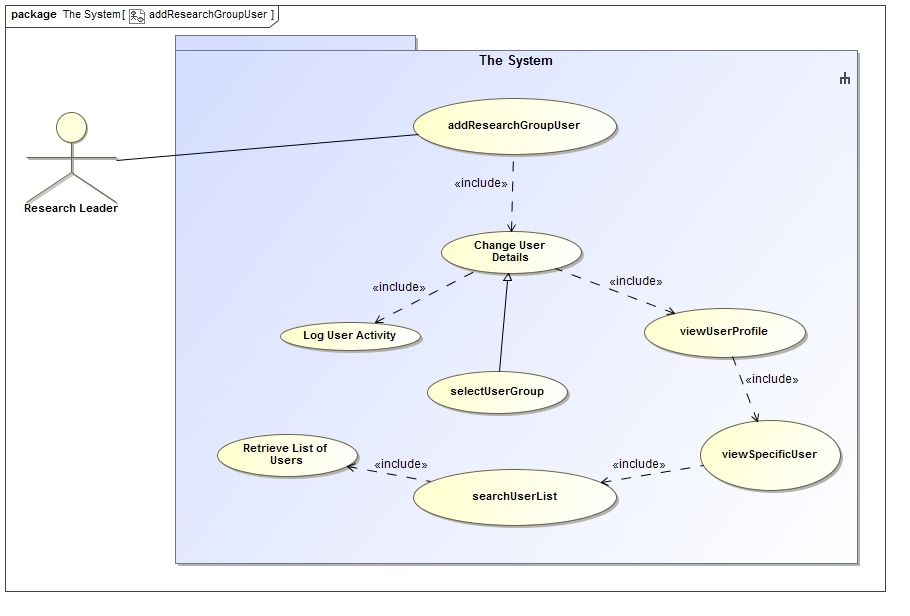
\includegraphics[width=1\textwidth]{req-func/uc__The_System__addResearchGroupUser.jpg}
\end{figure}

\begin{figure}[H]
    \centering
    \caption{Remove Research Group User}
    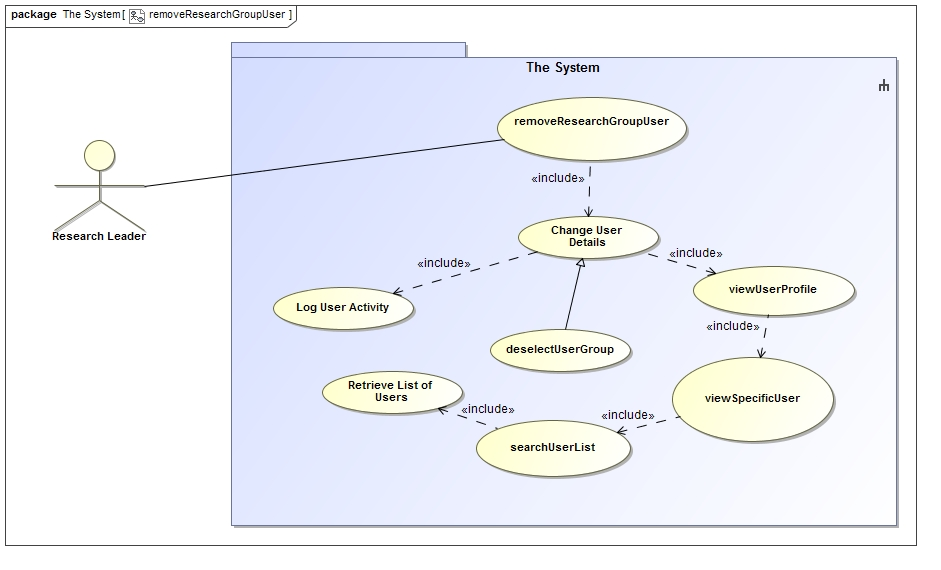
\includegraphics[width=1\textwidth]{req-func/uc__The_System__removeResearchGroupUser.jpg}
\end{figure}

\begin{figure}[H]
    \centering
    \caption{View Research Group Progress}
    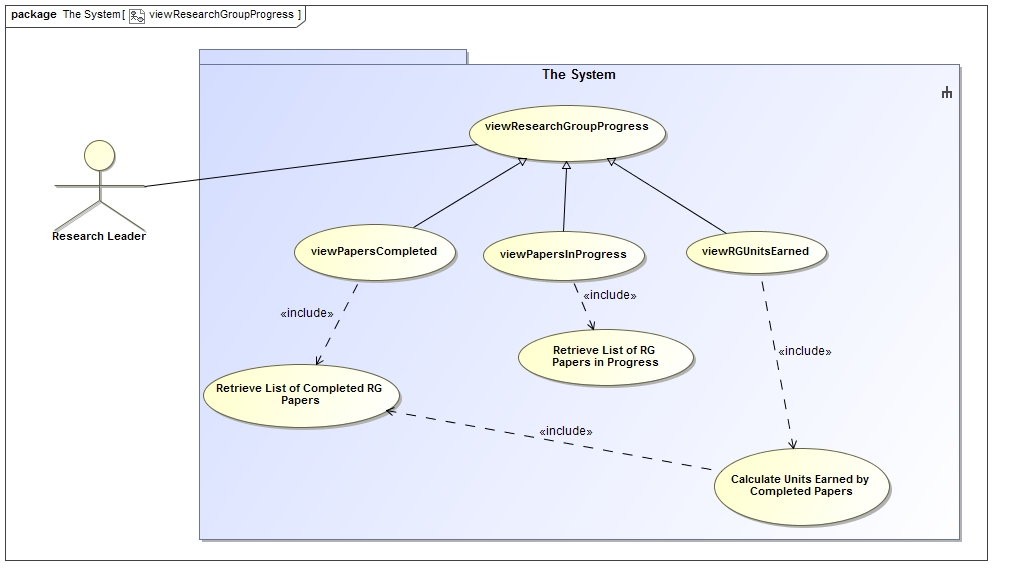
\includegraphics[width=1\textwidth]{req-func/uc__The_System__viewResearchGroupProgress.jpg}
\end{figure}

\begin{figure}[H]
    \centering
    \caption{View Research Group Users}
    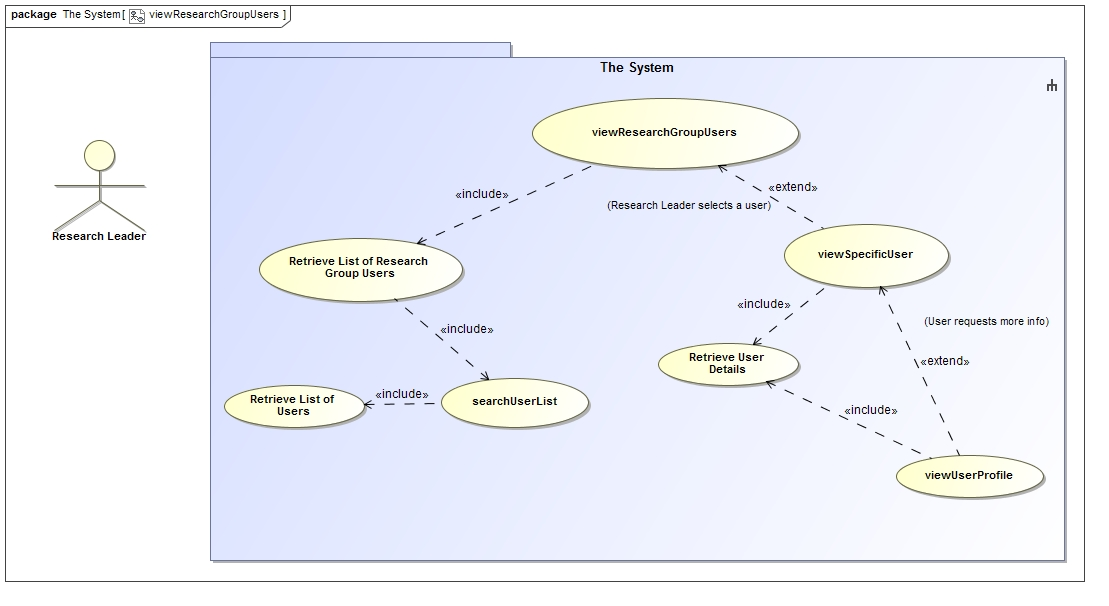
\includegraphics[width=1\textwidth]{req-func/uc__The_System__viewResearchGroupUsers.jpg}
\end{figure}

\begin{figure}[H]
    \centering
    \caption{View Units Earned}
    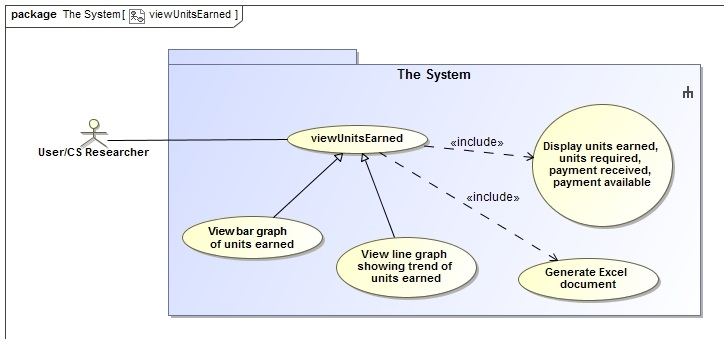
\includegraphics[width=1\textwidth]{req-func/uc__The_System__viewUnitsEarned.jpg}
\end{figure}

\begin{figure}[H]
    \centering
    \caption{Edit Profile}
    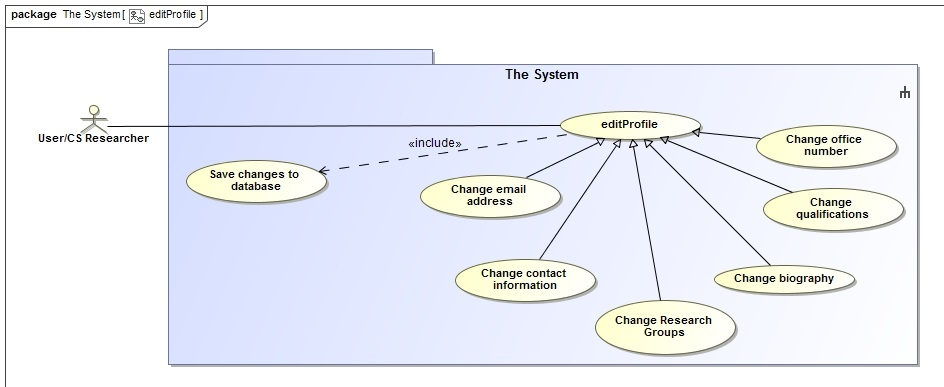
\includegraphics[width=1\textwidth]{req-func/uc__The_System__editProfile.jpg}
\end{figure}

\begin{figure}[H]
    \centering
    \caption{View Profile}
    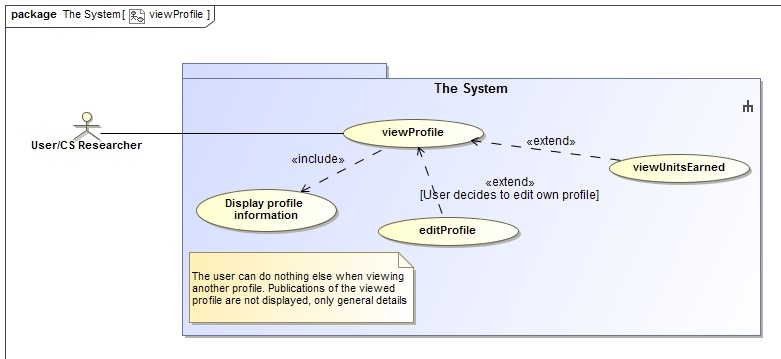
\includegraphics[width=1\textwidth]{req-func/uc__The_System__viewProfile.jpg}
\end{figure}

\begin{figure}[H]
    \centering
    \caption{View All Users}
    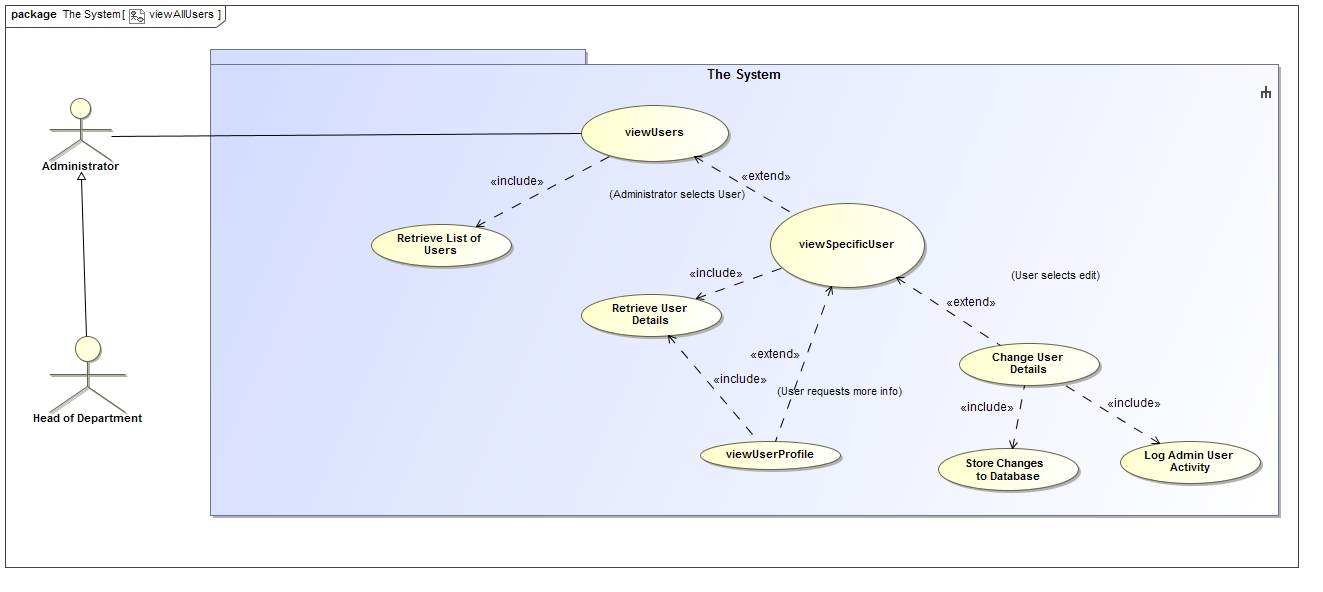
\includegraphics[width=1\textwidth]{req-func/uc__The_System__viewAllUsers.jpg}
\end{figure}

\begin{figure}[H]
    \centering
    \caption{Log In}
    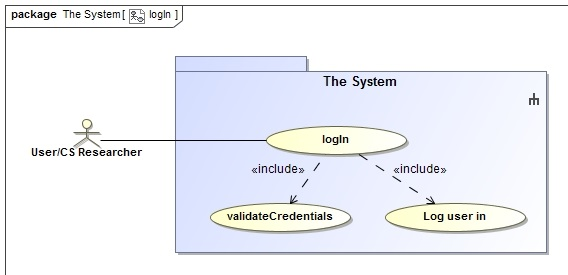
\includegraphics[width=1\textwidth]{req-func/uc__The_System__logIn.jpg}
\end{figure}

\begin{figure}[H]
    \centering
    \caption{Log Out}
    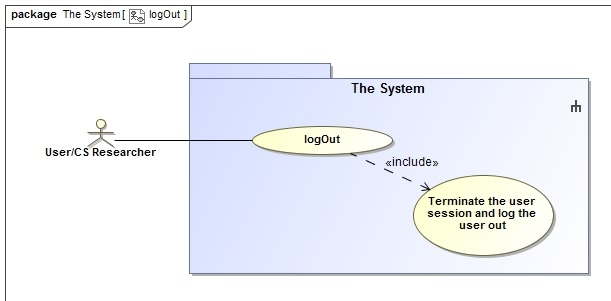
\includegraphics[width=1\textwidth]{req-func/uc__The_System__logOut.jpg}
\end{figure}

\begin{figure}[H]
    \centering
    \caption{View Activity Log}
    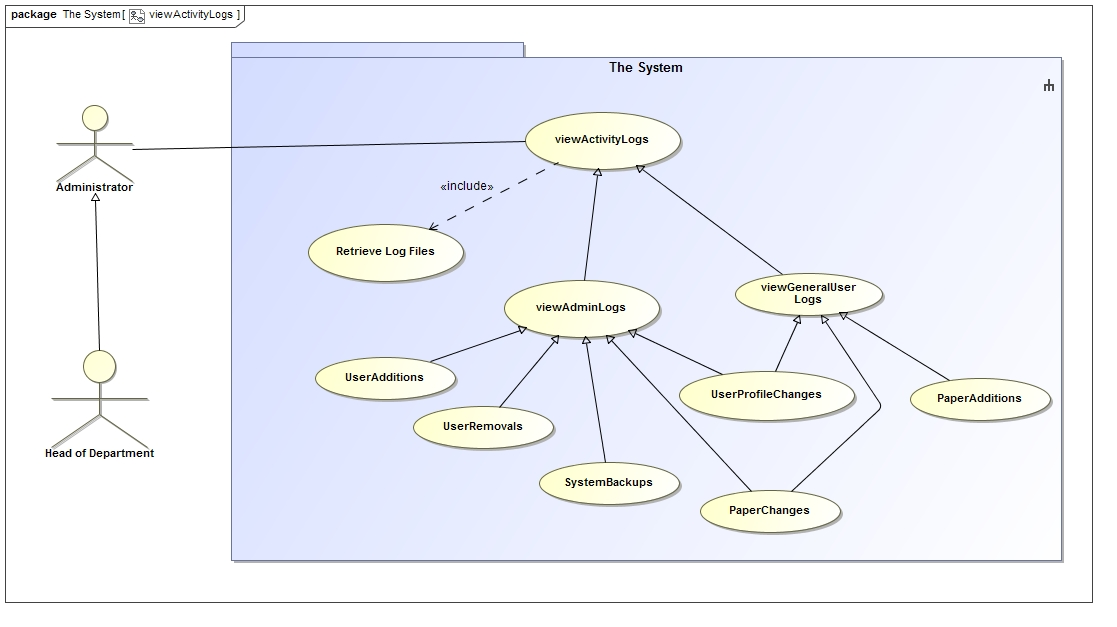
\includegraphics[width=1\textwidth]{req-func/uc__The_System__viewActivityLogs.jpg}
\end{figure}

\begin{figure}[H]
    \centering
    \caption{Back Up System Info}
    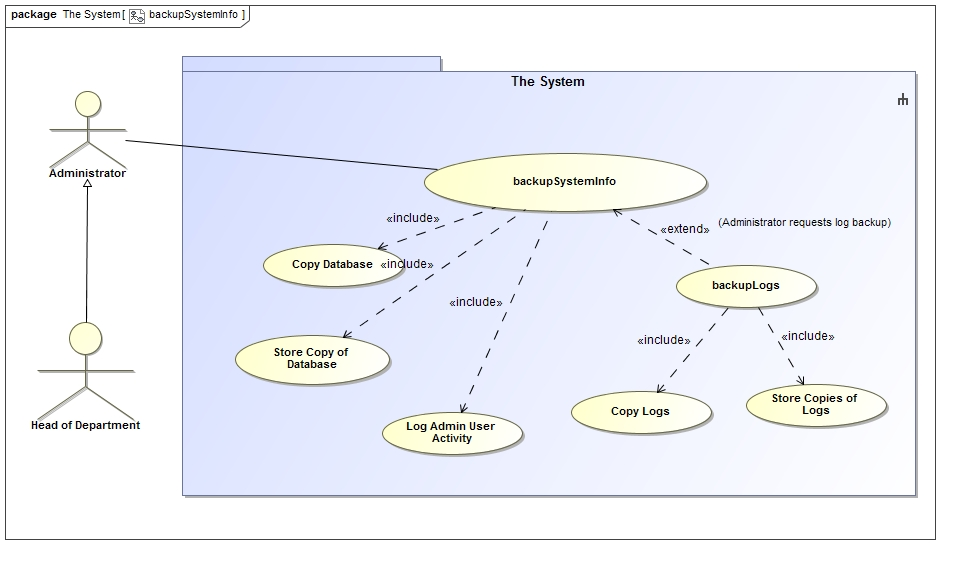
\includegraphics[width=1\textwidth]{req-func/uc__The_System__backupSystemInfo.jpg}
\end{figure}

%----------------------------------------------------------------------------------------
% Done by: Jedd Schneier and Josef Alberts (compiled by Gian Paolo Buffo)
%----------------------------------------------------------------------------------------
\newpage
\subsection{Process specifications}

This section illustrates the requirements around processes in the system which need to be followed. Activity diagrams are used to illustrate these process specifications.

\begin{figure}[H]
    \centering
    \caption{Log In}
    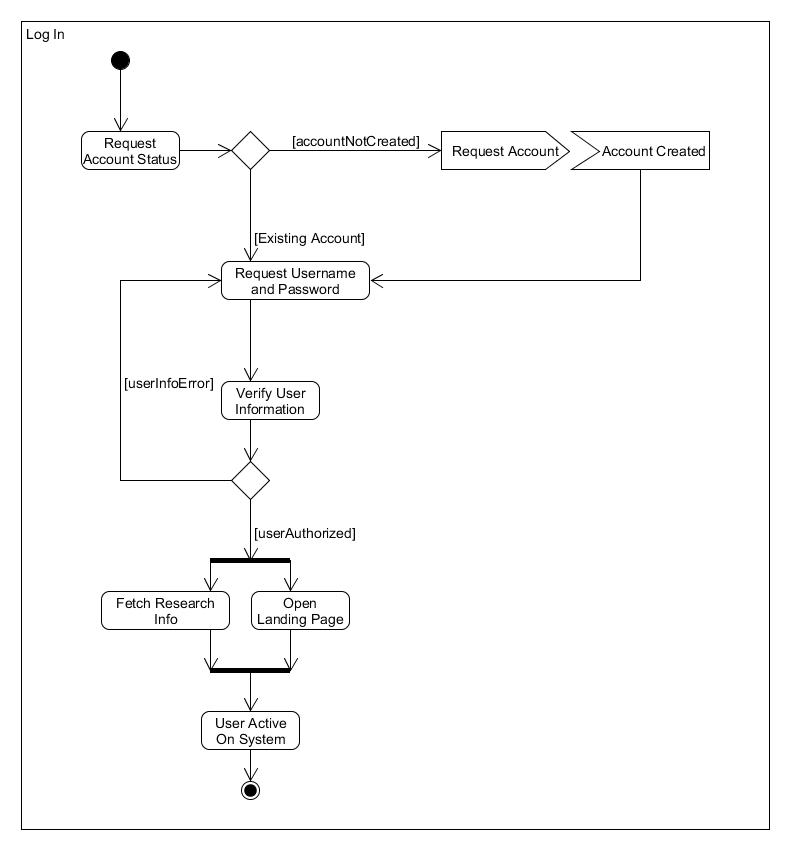
\includegraphics[width=1\textwidth]{process-spec/Activity_Login.jpg}
\end{figure}

\begin{figure}[H]
    \centering
    \caption{Add Paper}
    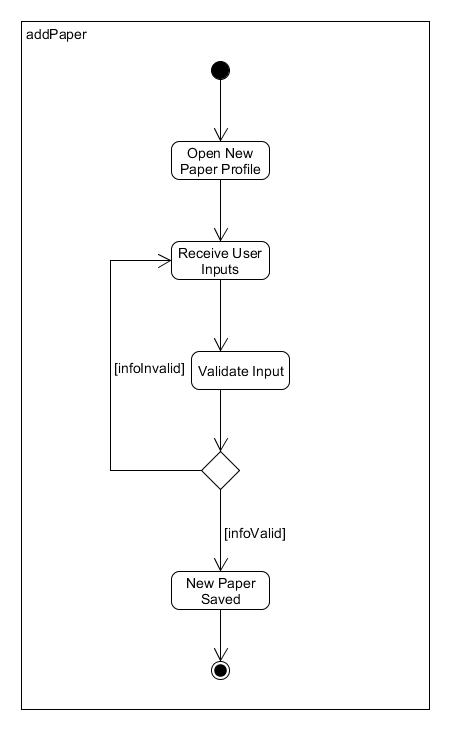
\includegraphics[width=1\textwidth]{process-spec/Activity_AddPaper.jpg}
\end{figure}

\begin{figure}[H]
    \centering
    \caption{Edit Paper}
    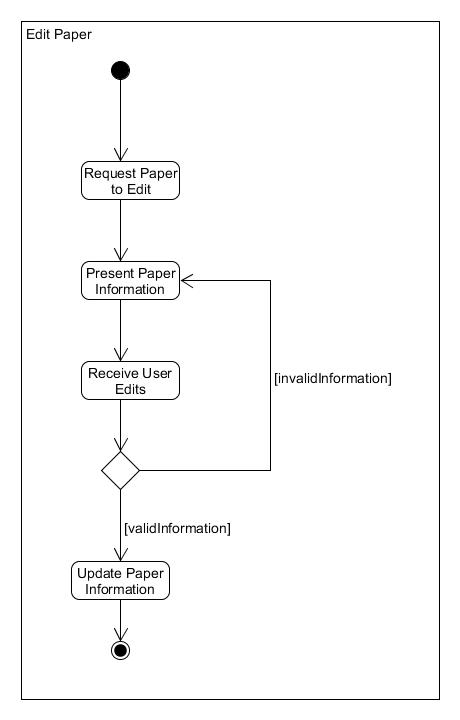
\includegraphics[width=1\textwidth]{process-spec/Activity_EditPaper.jpg}
\end{figure}

\begin{figure}[H]
    \centering
    \caption{Generate Report}
    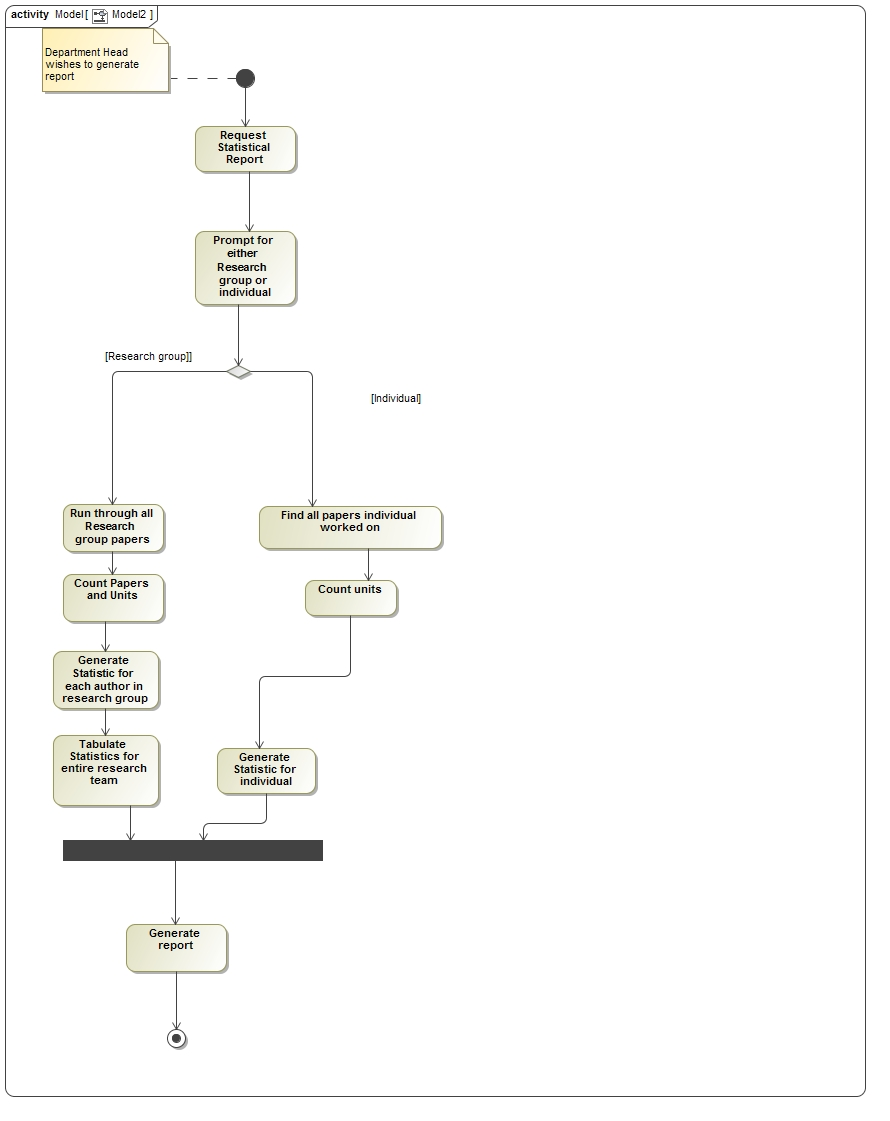
\includegraphics[width=1\textwidth]{process-spec/generateReportActivityDiagram.jpg}
\end{figure}

\begin{figure}[H]
    \centering
    \caption{Log Out}
    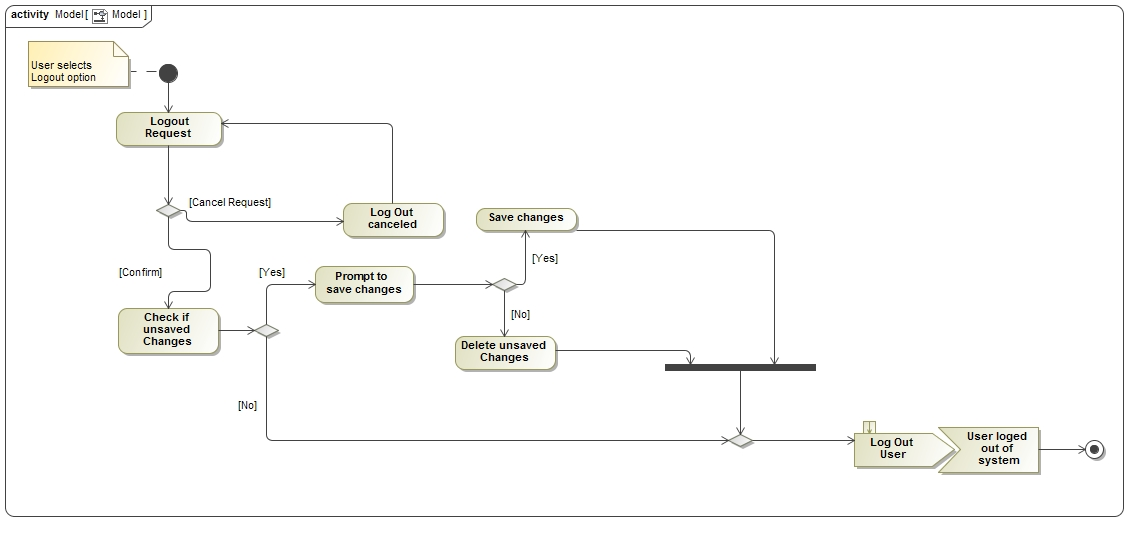
\includegraphics[width=1\textwidth]{process-spec/logOutActivityDiagraml.jpg}
\end{figure}

%----------------------------------------------------------------------------------------
% Done by: Kudzai Muranga and Sandile Khumalo (compiled by Gian Paolo Buffo)
%----------------------------------------------------------------------------------------
\newpage
\subsection{Domain Model}

In this section, the data structure requirements of the system are specified in a technology neutral way, by making use of UML class diagrams.

\begin{figure}[H]
    \centering
    \caption{Domain Model}
    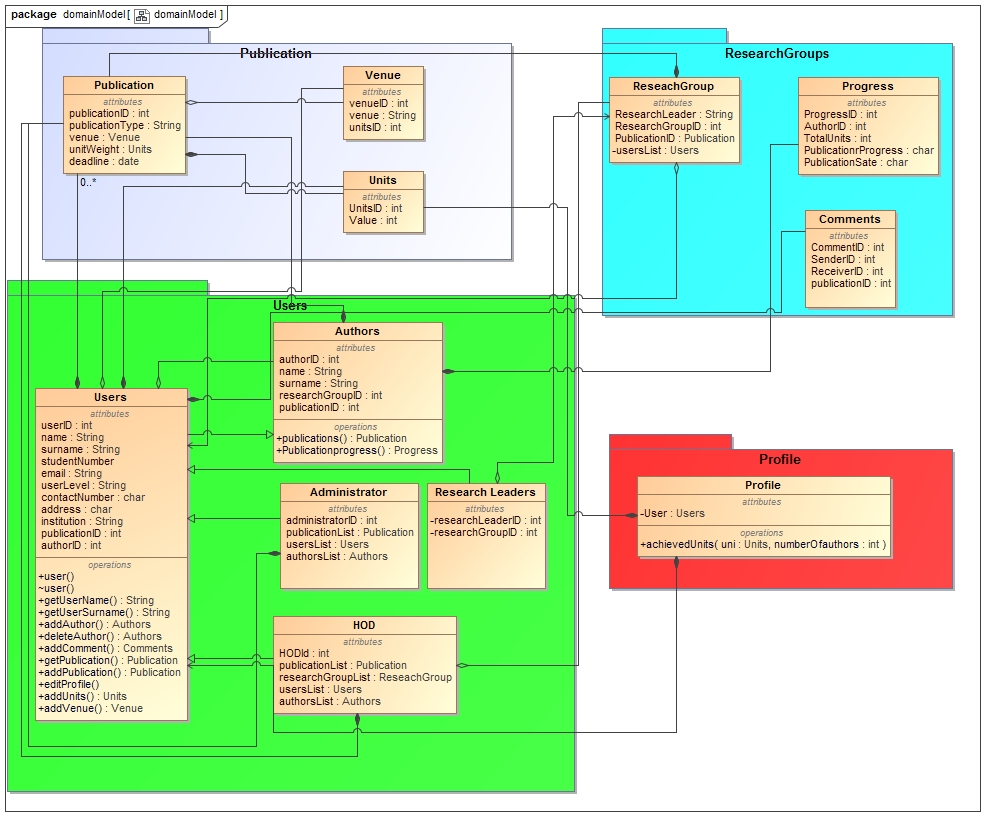
\includegraphics[width=1\textwidth]{domainModel.jpg}
\end{figure}


\newpage
\section{Software Architecture}
%----------------------------------------------------------------------------------------
% Done by: Jacques van Wyk (edited by Gian Paolo Buffo)
%----------------------------------------------------------------------------------------
\subsection{Architectural Patterns or Styles}
	Our research team has decided to use the MVC (Model-View-Controller)- and
	Layering architectural patterns for the research publication system for the mini
	project. Since the system should have a web-interface and a mobile Android interface,
	it is necessary to divide the system into parts where the two interfaces are independent
	of each other, but both can have concurrent access to a central database. In addition,
	this is necessary, because the interfaces will likely use different client-side
	technologies for the graphical user interface and client logic.
	\newline
	\newline
	The structure of MVC in the system:
	\begin{itemize}
		\item Model
		\begin{itemize}
			\item[] The Model represents the database and how the user and research
			data is structured, organized and stored in the database on the server-side. Furthermore, it provides an interface through the written server
			software by which the model can be manipulated from user interaction
			through the controller.
		\end{itemize}
		\item Controller
		\begin{itemize}
			\item[] The controller partly represents the logic and the user-functionality
			of the system and is downloaded or exists on the client's side of the
			system. The controller interfaces with the model and the view
			where the controller;for example, verifies user-input and determines the validity
			of it; consequently, the controller manipulates the model through
			the server-side software interface and the user's view is updated
			with the updated data stored in the model.
		\end{itemize}
		\item View
		\begin{itemize}
			\item[] The view represents the GUI(Graphical User Interface) that is displayed
			to the user and how it looks to the user when he/she interacts with it.
			The view gets updated when the model has been manipulated by some user's
			interaction with the controller.
		\end{itemize}
	\end{itemize}
	The MVC architectural pattern simplifies and modularizes the design of the research
	publication system in the following way:
	\begin{itemize}
		\item[-] The GUI's of the website- and Android applications can be developed
	  	independent from each other.
	  	\item[-] The client-side software and functionality of the website- and Android
	  	applications can be developed independent from each other.
	  	\item[-] The database and server software can be developed independent from which
	  	client-side programming languages will be used and can be redistributed
	  	to work with other controllers and views.
	\end{itemize}
	The Layering architectural pattern makes use of a set of programmed layers. Each
	layer has been implemented to provide a certain unique functionality and can be used or
	reused by certain other layers.
	By making use of the Layering architectural pattern it can make the development
	life cycle of the research publication system more efficient in the following ways:
	\begin{itemize}
		\item[-] Layers can be tested and debugged individually.
	  	\item[-] Layers can be reused in other layered systems.
	  	\item[-] Layers can be updated and improved to replace the older ones.
	  	\item[-] Layers can be used to improve the security of the system; for example,
	  	all user-input must go through a security layer before it can be transmitted
	  	to other layers.
	  	\item[-] Layers can help the system to be formed as a united whole.
	  	\item[-] Layers helps the development of the system to be less complex, because
	  	the functionality is integrated into their separate layers to be worked on separately.
	\end{itemize}
	Examples of layers that can be used in the research publication system:
	\begin{itemize}
		\item[-] A client-handler layer to handle what happens with user-input. Two different
	  	client-handlers might be implemented for web- and Android applications.
		\item[-] A display-handler layer to receive data from a data source and view it to the 	        user in an appealing manner. Two different display-handlers might be implemented for
	  	web- and Android applications.
		\item[-] A security-handler layer to verify user-input or file-uploads before it
	  	transfers it to the server.
		\item[-] A server-handler to modify the database or to retrieve data from the
	  	database.
		\item[-] etc.
	\end{itemize}
%----------------------------------------------------------------------------------------
% To be done by: Hlengekile
%----------------------------------------------------------------------------------------
\subsection{Architectural Tactics or Strategies}

%----------------------------------------------------------------------------------------
% To be done by: Jason and Sandile (edited by Gian Paolo Buffo)
%----------------------------------------------------------------------------------------
\subsection{Use of Reference Architectures and Frameworks}
The reason we are using reference architectures in this system is due to the fact that it helps with the development process of the system. What this section is meant to include is how the system should use frameworks to implement the architectural pattern(s) chosen and what the reasons for using these frameworks are.

\subsubsection{Web 2.0 Reference Architecture}
\noindent
We have chosen to use and refer to the Web 2.0 reference architecture due to the fact that this is primarily a web-based system. The Web 2.0 Reference Architecture can be found here: \url{http://archive.oreilly.com/pub/a/web2/excerpts/web2-architectures/chapter-5.html}.\\

\noindent
This Reference Architecture has 4 main tiers that are essential to our system, namely:
\begin{enumerate}
	\item Resource Tier
	\item Client Tier
	\item Service Tierand
	\item Design, Development and governance tools
\end{enumerate}

\subparagraph{Resource Tier}\hspace{-10pt}:\\
The Resource tier includes `backend systems that can support services that will be consumed over the internet'. Thus our system will need to use this tier to ``consume" information which is input by the user for either: signing up, logging in adding a paper, changing the state of a paper, removing a user, adding a user etc. All this information will be updated in the database (also considered to be the model of the MVC pattern) which will store all the data of the user's and metadata of the paper's. This tier directly links with the Service tier due to the fact that for validation and storage of the input it needs to be sent to the server side and validated and stored from there. 

\subparagraph{Client Tier}\hspace{-10pt}:\\
This component helps the user to use services and display graphical views. These are the web browsers used.

\subparagraph{Server Tier}\hspace{-10pt}:\\
This component connects the resource tier. Since they will be two versions of the application a web based and a android app, we will use the adapter architecture to read the data.


\subparagraph{Design, Development and Governance Tools}\hspace{-10pt}:\\
This tier refers to the tools that are used to actually build the web application. The reference architecture refers specifically to IDE's however I disagree with that in that one does not necessarily need an IDE to built a web application. This does not necessarily fit into this reference architecture directly. It is more just used to describe a tool for the developer to use and does not use the other tiers directly.
\subsubsection{Django}Django is another framework will be used. The reason for this is that it follows the MVC architecture design pattern .Django’s primary goal is to make it easy to create data driven websites that are complex. It comes with caching to make processing of data that is frequently uses faster. Django being a server side helps in keeping information safe. In addition Django is very fast.
\subsubsection{Bootstrap}We will use bootstrap cs to style the web interface of System .Advantages of using bootstrap  is that is customizable, you pick and choose the feature you want then download the files. Another advantage of bootstrap is that is responsive. This will help other mobile devices such as IOS and blackberry which aren’t running on the specified android app that will be designed. Bootstrap enhances working together as a group because it brings consistency regardless of who did the work and it stays the same across all browsers. Bootstrap is consistently updated so it stays in synced with new technologies. It also has a large support community in case you run into problems.\par 
\subsubsection{Android SDK}Android SDK will be used to develop the android app, this is specifically developed for android so t makes the functionality of the app faster than an app developed using hybrid frameworks.(such as ionic).\par
\subsubsection{AngularJS}Another framework to be used is AngularJS. AngularJS enables massive parallel development. It also reduces code length, making code easier to maintain. Loops that could have been long are reduced to a single line. It allows a developer to deal with modules on the client side as they would deal with them on the server side.\par  


\subsubsection{jQuery Mobile Framework}
jQuery Mobile is a multi-platform mobile `touch-optimized web framework'. This can be used to develop the Android application for the system. This framework allows a developer to design one application that will be able to run on all smartphone and tablet OS's, allowing for easy portability, if needed at a later stage. To develop an application using this framework, developers need to use web-based languages such as: jQuery, HTML, CSS. It does allow for client-server communication (which is what is needed for this system). This framework is based on web development but was written specifically for smartphone and tablet applications and websites. jQuery mobile uses device-level optimizations to make sure that the layout is appropriate for the specific device it is running on. This allows for easier development of a device agnostic application. This framework is also extensible. It allows for many different third party plugins and is integrable with other frameworks such as AngularJS, Backbone.js and mobile frameworks (to name a few). This creates an opportunity to easily integrate frameworks which can implement the MVC architectural pattern, which is what is being used to develop this system.

\subsubsection{Backbone.js}
This framework would be used together with the Android application to provide the missing JavaScript architecture which jQuery Mobile cannot provide. jQuery allows the implementation of multiple patterns with a Model and View which is referred to MV*. Thus the implementation of the MVC architectural pattern is possible, which is the pattern that will be used in this system. Backbone helps to structure the application (which could be complex) while still keeping it easily maintainable and fast. Backbone is lightweight and performance-wise it is very good due to the fact that it prefers to integrate with other frameworks to create a User Interface rather than it having something built into it for this feature, thus reducing overhead. The reason that Backbone would be used with jQuery Mobile is the fact that Backbone is not used to create a UI (i.e. the View is basically just a template). Backbone may not necessarily implement a strict class system but it does use prototype-based inheritance as well as object extensions. This makes it possible to implement architectural and design patterns which use Object-Oriented programming.

\subparagraph{Jackbone.js:}
Since the integration of jQuery Mobile and Backbone is common they decided to create a framework that integrates the two and makes it easier to develop lightweight, extensible and fast mobile applications. It also makes it easier to implement MV* patterns such as MVC. Where Backbone did not necessarily have a Controller, Jackbone has extended the Backbone framework to implement a controller in the MVC pattern. It relies mostly on Backbone.js and provides specialised classes for view and router.

%----------------------------------------------------------------------------------------
% Done by: Josef & GP
%----------------------------------------------------------------------------------------
\subsection{Access and Integration Channels}
In this section we mention and discuss the main access and integration channels of this system. Among them are different human users, each acting in different roles, and system users - such as remote clients or the database software.
\begin{itemize}
\item \textbf{Human Users:}
Human users will have access to the platform though two separate channels. Namely, through a website interface and a native Android application. 
\begin{itemize}
\item \textbf{Administrator:} Two administrator users will have access to the system. Firstly the Head of Department will have an administrator account through which he will have access to all features, and all data, in the system. He will, therefore, be able to access and update information on papers without having to be an author on the paper. He will also have access to the database on which all system data (including users, papers and venues) is stored. This will require that such access is available on both the web interface and the Android app. Additionally there will be another administrator account through which a technician must access the system in order to conduct routine maintenance and fix possible errors.
\item \textbf{User:} User accounts will be allowed to add papers to the system as well as edit papers which they are already assigned to (either as Authors or not). Users do not have administrative access to any data (apart from Authors and Venues) which they have not been assigned to. For instance, a User may not view or edit a paper which they have not been assigned to by another User, already assigned to said paper.
\item \textbf{Author:} Authors have no access to this system. Authors are simply data entries in the database which have been stored to simplify data entry in cases where an author needs to be assigned to several papers.
\end{itemize}
\item \textbf{System Users:}
The system will be sharing information to the two main portals - being web and Android. In order to accomplish this we will be implementing an API (Application Program Interface) which will act as a layer of abstraction. It will provide access to requested information (users, papers, venues, searches, etc.) and carry out tasks on behalf of the portal (be it web or Android). By doing this we will be advancing flexibility of the system, since the same API calls will be used regardless of the platform used to make them. The API will function by receiving a call, delegating the call to the server and then forwarding the response to the client (who made the initial request).

Furthermore the database will be accessed via MongoDB's built-in API and called from the server - where each call from the client is handled. In other words, the server is accessed by a client interface and the server software, in turn, accesses the database.

\item \textbf{Protocols:}
Here we discuss some of the main protocols we plan to use in implementing this system. This includes protocols for transferring miscellaneous data (such as status codes or images) as well as data such as emails or hypertext files.
\begin{itemize}
\item \textbf{TCP/IP (Transmission Control Protocol/Internet Protocol):}
TCP/IP will be used to establish connections between computers such as the server and the clients. TCP allows us to open a data stream to which we can read and write. This allows us to transfer data over networks, including the Internet. We chose TCP over alternatives such as UDP due to its inherent reliability.

\item \textbf{HTTP (HyperText Transfer Protocol):}
HTTP will be used to initiate transfers between components of the system. GET and POST request will be used to transfer data to and from the server, database and the numerous client interfaces. Additionally, HTTP provides us with built-in error codes which will allow the system to track the success or failure of a request and react accordingly (retrying or requesting new input data from user).

\item \textbf{SMTP (Simple Mail Transfer Protocols):}
SMTP will be used to send emails to users, notifying them of oncoming deadlines for paper submission. SMTP provides a stable method to transfer email by letting us transfer the email to a SMTP server and then queueing the mail until the next server - either an intermediate SMTP or POP3/IMAP server - becomes available. By using SMTP we will minimize the chance of mail getting lost and a user not being notified.

\item \textbf{FTP (File Transfer Protocol):}
FTP will be used to transfer files (such as HTML, CSS or PHP files) to and from the server. It will specifically be used in transferring files to the webserver from remote locations.


\end{itemize}

\end{itemize}
%----------------------------------------------------------------------------------------
% To be done by: Jedd
%----------------------------------------------------------------------------------------
\subsection{Technologies}

%----------------------------------------------------------------------------------------
% Done by: Jacques van Wyk and Jason Gordon
%----------------------------------------------------------------------------------------
\newpage
\section{Open Issues}

\begin{itemize}	
\item Should the admin be able to edit the meta-data of the papers or not?
	\begin{itemize}
	\item Should the research leader be able to edit the meta-data of papers in their research group?
	\end{itemize}
\item What server will be used to host our site? 
\item Should we add any backup capabilities for the database?
	\begin{itemize}
	\item If so, will the admin be the only one able to backup the database?
	\end{itemize}
\item Is there a specific database that we need to use to store the information (i.e. MySQL, MongoDB, Neo4j etc.)?
\item Should the system be able to support more than 100 users if, for example, another employee was employed by the Computer Science Department? (i.e. should the addition of users past 100 be allowed?)
\item Should any user be able to add papers on behalf of other users? There may be risks involved when allowing this.
\item If a new user is added and they are already an author of a paper (when they were not a user of the system) should the papers, which the new user is part of, be displayed on their profile?
	\begin{itemize}
	\item Will this new user receive units for the paper if it has already been published?
	\end{itemize}
\item If a paper has been ``terminated`` should the metadata still be editable while it is in a terminated state (besides for changing the state of the paper)?
\end{itemize}


\end{document}
